% Autor: Manuel Lippert
% Physikalisches Praktikum

% Main-Datei für die Auswertung in TeX

% Struktur:
% Jedes Kapitel hat einen Input-File. Um Merge-Konflikte zu verhindern wird angeraten für jede 
% Datei eine eigene Tex Datei zu machen und sie im jeweiligen Kapitel zu importieren. Die in
% Input-Struktur dient zur besseren Übersicht und für mögliche Ordner, welche hier vorhanden sind. Die Zahlen vor den 
% Ordner dient zur Ordnung der einzelnen tex-Files nach Kapiteln


% Packages
\documentclass[paper=a4,bibliography=totoc,BCOR=10mm,twoside,numbers=noenddot,fontsize=11pt]{scrreprt}
\usepackage[english]{babel}
\usepackage[T1]{fontenc}
\usepackage[latin1, utf8]{inputenc} %ä, ö, ü inbegriffen
\usepackage[babel,german=quotes]{csquotes} %For Quotes
\usepackage{lmodern}
\usepackage{graphicx}
\usepackage{nicefrac}
\usepackage{fancyvrb}
\usepackage{amsmath,amssymb,amstext}
\usepackage{siunitx}
\usepackage{url}
\usepackage{natbib}
\usepackage{microtype}
\usepackage[format=plain]{caption}
\usepackage{physics}
\usepackage{titleref} 

% Zusätzliche Packages
\usepackage{geometry} % Verändert Seitengeometrie
\usepackage{anyfontsize} % Alle Schriftgrößen möglich machen
\usepackage[table]{xcolor} % Farbliche Gestaltung Tabellen
\usepackage{ifthen} % Für kompliziertere tex-Files
\usepackage[absolute,overlay]{textpos} %Textboxen
\usepackage{amsfonts} % Schriftarten
\usepackage{xstring} % Stringoperationen
\usepackage{tikz} % Zeichnungen
\usepackage{pdfpages} % Import von pdfs (Protokolle)
\usepackage{hyperref} % Verlinkungen im Dokument
\usepackage{makecell} % Zeilenumbruch in Zelle

% Abschnittseinrückung und -abstand
% Die folgenden Zeilen sollen möglichst nicht verändert werden
\parindent 0.0cm
\parskip 0.8ex plus 0.5ex minus 0.5ex

% Anzahl und Größe von Gleitobjekten
% maximal 2 Objekte oben und unten
% erlaubt auch größere Bilder, welche die ganze Seite benötigen
% Die folgenden Zeilen sollen möglichst nicht verändert werden
\setcounter{bottomnumber}{2}
\setcounter{topnumber}{2}
\renewcommand{\bottomfraction}{1.}
\renewcommand{\topfraction}{1.}
\renewcommand{\textfraction}{0.}

%\sc und \bc veraltet. Daher: (20.09.2018)
\DeclareOldFontCommand{\sc}{\normalfont\scshape}{\@nomath\sc}
\DeclareOldFontCommand{\bf}{\normalfont\scshape}{\textbf}

% Verschiedenes
\pagestyle{headings}          % Der Seitenstil sollte möglichst nicht verändert werden
\graphicspath{{./Bilder/}}    % Der Pfad für die Abbildungen Abbildungen wird gesetzt
\VerbatimFootnotes            % \verb etc. auch in \footnotes mφglich

% Funktionen
\newcommand\tab[1][1cm]{\hspace*{#1}}
\newcommand{\vect}[1]{\boldsymbol{\mathbf{#1}}}
\newcolumntype{g}{>{\columncolor[rgb]{ .741,  .843,  .933}}l}
% Tiefgestellte Zahlen nicht kursiv
\catcode`_=\active
\newcommand_[1]{\ensuremath{\sb{\mathrm{#1}}}}

\begin{document}

    \nonfrenchspacing

    % 0.Chapter Cover
    % 0. Cover

% Hier sind nur die Variablen und der Abschnitt Informationen (unten) zu bearbeiten der REst läuft automatisch ab (z.b Farbenänderung)

% Noch abänderbar nur ein Vorschlag
\newgeometry{top=30mm, bottom=20mm, inner=20mm, outer=20mm}
\thispagestyle{empty}

% Colors (Notability Colors)
\definecolor{Notablue}{HTML}{3498DB}		
\definecolor{Notared}{HTML}{CF366C}			
\definecolor{Notagreen}{HTML}{19B092}		
\definecolor{Notaorange}{HTML}{FA9D00}		
\definecolor{Notagrey}{HTML}{969696}		
\definecolor{Notalavendel}{HTML}{9DBBD8}	

% Boolean by default false. Für Absatz in der Überschrift
\newboolean{twoRows}
\newboolean{symbol}

% Funktions
\makeatletter
   \def\vhrulefill#1{\leavevmode\leaders\hrule\@height#1\hfill \kern\z@}
\makeatother
\newcommand*\ruleline[1]{\par\noindent\raisebox{.8ex}{\makebox[\linewidth]{\vhrulefill{\linethickness}\hspace{1ex}\raisebox{-.8ex}{#1}\hspace{1ex}\vhrulefill{\linethickness}}}}

% Variables
\def\schriftgrosse{40}
\def\linethickness{1,5pt}

\def\farbe{black}
\def\fach{PPBphys2}
\def\name{Manuel Lippert - Paul Schwanitz}
\def\titel{Förster-\\[0,5cm] Resonanzenenergietransfer \\[0,5cm] an biologischen Proben} % Absatz mit \\[0,5cm]
\def\bottom{WS2021/22}
\def\datum{28.09.2021}
\def\platz{NWI | BT5.3}
\def\betreuer{Chenyu Jin}

\def\teilnehmerm{Manuel Lippert}
\def\emailm{Manuel.Lippert@uni-bayreuth.de}
\def\teilnehmerp{Paul Schwanitz}
\def\emailp{Paul.Schwanitz@uni-bayreuth.de}

%\def\auswertp{}
%\def\messp{}
%\def\protop{}

\def\groupnr{11}

\begin{titlepage}
			
	\centering
	{\LARGE \sffamily {\textbf{\bottom}\par}}
	\vspace{2,5cm}
    {\fontsize{30}{0}\sffamily\ruleline{\textcolor{\farbe}{\textbf{\fach}}}\par}
    \vspace{6cm}
	{\Large\sffamily \ruleline{\name}\par}
		
	\IfSubStr {\titel} {\\[0,5cm]} {\setboolean{twoRows}{true}} {\setboolean{twoRows}{false}}
	
	\ifthenelse{\boolean{twoRows}}
		{
			\begin{textblock*}{21cm}(0cm,7,8cm) % {block width} (coords), centered		
				{\fontsize{\schriftgrosse}{0}\sffamily\textcolor{\farbe}{\textbf{\titel}}\par}
			\end{textblock*}
		}
		{
			\begin{textblock*}{21cm}(0cm,9cm) % {block width} (coords), centered		
				{\fontsize{\schriftgrosse}{0}\sffamily\textcolor{\farbe}{\textbf{\titel}}\par}
			\end{textblock*} 
		}
	
	% Choose Logo
	\ifthenelse {\equal{\farbe}{Notared}} {\def\logo{Bilder/Logo/UniBTNotared}}
		{\ifthenelse {\equal{\farbe}{Notagreen}} {\def\logo{Bilder/Logo/UniBTNotagreen}}
			{\ifthenelse {\equal{\farbe}{Notablue}} {\def\logo{Bilder/Logo/UniBTNotablue}}
				{\ifthenelse {\equal{\farbe}{Notaorange}} {\def\logo{Bilder/Logo/UniBTNotaorange}}
					{\ifthenelse {\equal{\farbe}{Notagrey}} {\def\logo{Bilder/Logo/UniBTNotagrey}}
						{\ifthenelse {\equal{\farbe}{Notalavendel}} {\def\logo{Bilder/Logo/UniBTNotalavendel}}	
							{\ifthenelse {\equal{\farbe}{black}} {\def\logo{Bilder/Logo/UniBT}}	
								{\def\logo{noLogo}}
							}
						}
					}
				}
			}
		}	

	\IfSubStr{\logo}{noLogo}{\setboolean{symbol}{false}}{\setboolean{symbol}{true}}
	
	% Gruppe
	\vspace{10cm}
	{\large\sffamily{Gruppe \groupnr}}
	
	%Logo
	\vfill

	\ifthenelse{\boolean{symbol}}
		{
			\begin{figure}[h]
			\begin{center}
				
				\includegraphics[width=2cm]{\logo}
				
			\end{center}
			\end{figure}
		}
	
\end{titlepage}

\restoregeometry

% Information
\chapter*{Informationen}
\label{chap:info}

\begin{tabular}{l l}

	{\textbf{Versuchstag}} \hspace{1cm} & \hspace{1cm} {\datum}\\[0,2cm]
	{\textbf{Versuchsplatz}} \hspace{1cm} & \hspace{1cm} {\platz}\\[0,2cm]
	{\textbf{Betreuer}} \hspace{1cm} & \hspace{1cm} {\betreuer}\\[1,2cm]
	{\textbf{Gruppen Nr.}} \hspace{1cm} & \hspace{1cm} {\groupnr}\\[0.2cm]
	% Für Fortgeschittenenen Praktikum
	{\textbf{Teilnehmer}} \hspace{1cm} & \hspace{1cm} {\teilnehmerm~(\emailm)}\\[0.2cm]
		     			  \hspace{1cm} & \hspace{1cm} {\teilnehmerp~(\emailp)}\\[0.2cm]
	% Für Grundpraktikum
	%{\textbf{Auswertperson}} \hspace{1cm} & \hspace{1cm} {\auswertp}\\[0.2cm]
	%{\textbf{Messperson}} \hspace{1cm} & \hspace{1cm} {\messp}\\[0.2cm]
	%{\textbf{Protokollperson}} \hspace{1cm} & \hspace{1cm} {\protop}\\[0.2cm]

\end{tabular}

    \thispagestyle{empty}
    \cleardoublepage
    \tableofcontents
    \cleardoublepage

    % 1.Chapter Instructions
    % 1. Introduction

\chapter{Introduction}
\label{chap:intro}

Spectroscopy is a very important tool to discover the structure from atoms and molecules. With the help of that tool, the physicists discover the spectral lines of the H-atom. This is where spectroscopy began. \\
The research in this are also helps to discover things like fine and hyperfine structure. What finaly leads to Quantum mechanics.\\
Furthermore, spectroscopy is also very useful tool for other areas of science like chemistry or biology. In this areas spectroscopy helps to analyze probes and provides information about which materials the probe is made of.\\
So the aim of this Experiment is to get in contact with experimental atom and nucleus physics by means of Doppler-free  Saturation Spectroscopy of Rubidium.

    % 2.Chapter Theorie
    % 2. Fragen zur Vorbereitung

\chapter{Theoretischer Hintergrund}
\label{chap:theo}
Bevor wir uns zur Versuchsdurchführung und der Auswertung zuwenden wollen wir die Theorie von FRET näher besprechen. Dafür verwenden wir \citep{Anleitung} und \citep{Fluorescence} als Hauptquelle.

\section{FRET-Effekt}
\label{sec:dipolToFRET}
Um den FRET-Effekt zu beobachten, werden zwei Farbstoffe benötigt mit unterschiedlichen Absorptions- und Emissionsspektrum. Dabei muss sich das Emissionsspektrum des \textbf{\textit{Donor}}-Farbstoffs und das Absorptionsspektrum des \textbf{\textit{Akzeptor}}-Farbstoffs eine deutliche Überlappung aufzeigen (hellblauer Bereich in Abb. \ref{image:lappung}).\\

Durch Anregung des Donors wird das Molekül von einem Grundzustand $S_0$ in den ersten angeregten Zustand $S_1$ gebracht. Anzumerken ist aber, dass Moleküle anders, wie bei einzelnen Atomen, mehrere Energiezustände haben, darunter fällt die Energie des elektronischen Übergangs, der Schwingung und der Rotation (Gesamtenergie $E=E_{rot}+E_{vib}+E_{el}$). Das Vorhandensein von mehreren Energiezuständen hat zur Folge, dass sich Unterniveaus bilden in Fall von Molekülen entsteht ein \textit{Bandspektrum}.
\begin{center}
    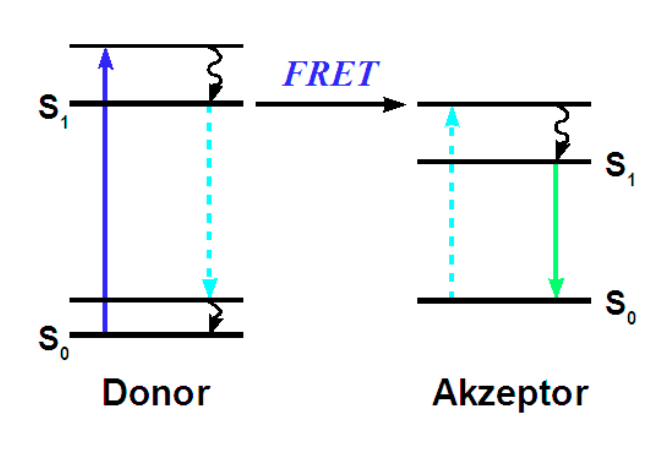
\includegraphics[scale=0.23]{FRET-Effekt.png}
    \captionof{figure}{FRET-Übergang \citep{Anleitung}}
    \label{image:FRET}
\end{center}
Durch Anregung eines Photons entsteht ein Übergang in das höhere Energieniveau $S_1$. Dieses koppelt sich an Vibrationen und verliert dabei ein Teil der Anregungsenergie des Photons. Nach der sogenannten Lebensdauer $\tau$ emittiert das Molekül spontan ein Fluoreszenzphoton und fällt in den Grundzustand $S_0$ zurück. Bei diesem Vorgang kommt es dann zur sogenannten \textit{Stokes-Verschiebung}, wodurch aufgrund des Energieverlusts die Wellenlänge des Fluoreszenzphotons höher ist als die des Anregungsphotons. Liegt nun die Wellenlänge des Fluoreszenzphotons im Absorptionsspektrum des Akzeptors geht die Anregungsenergie des Donors \textbf{\textit{strahlungslos}} auf den Akzeptor über, welcher wiederum durch Kopplung an Vibrationen ein Fluoreszenzphoton emittiert und in seinen Grundzustand zurückfällt. Diesen Vorgang nennt man \textbf{\textit{FRET-Effekt}} (siehe Abb. \ref{image:FRET}).
\newpage
\subsection*{Dipol-Dipol-Wechselwirkung und Fermis' goldene Regel}
Damit der Übergang der Energie strahlungslos vonstattengeht, muss es zu einer Dipol-Dipol.Wechselwirkung zwischen Donor und Akzeptor kommen. Dabei hängt die Effizienz des Energieübertrags von der Spektrenüberlappung, der Orientierung der Dipole und der Distanz der Farbstoffe verursacht vom Dipolfeld ab. Die Übergangswahrscheinlichkeit und die Effizienz des FRET-Effekts kann durch Fermis' goldene Regel angegeben werden:
\begin{gather}
    \abs{\left\langle \phi_{D}^* \phi_A \bigg \vert \frac{\kappa}{4\pi\epsilon_0} \frac{\mu_D\mu_A}{r^3} \bigg \vert \phi_D \phi_A^* \right\rangle }^2
\end{gather}
Dabei entspricht $\kappa$ dem winkelabhängigen Orientierungsfaktor der Dipole, $\epsilon_0$ der elektrischen Feldkonstante, $\mu_D$ dem elektrischen Dipolmoment des Donors und $\mu_A$ dem elektrischen Dipolmoment des Akzeptors. Die Abhängigkeit von $\frac{1}{r^3}$ kommt dabei von der Multipolentwicklung des Dipol-Moments und durch das quadrieren von Fermis' goldener Regel entsteht entsteht die $\frac{1}{r^6}$-Abhängigkeit in Gleichung \ref{eq:effizienz}. Die Effizienz des FRET-Effekts lässt sich dann wie folgt angeben:
\begin{gather}
    E = \frac{\text{Zahl der Energitransfers}}{\text{Zahl der Anregungen}} = \frac{k_{ET}}{k_F + k_{ET} + k_0} = \frac{R_F^6}{R_F^6+R^6}
    \label{eq:effizienz}
\end{gather}
Hierbei entspricht $R_F$ dem Försterradius und $R$ den Abstand zwischen den beiden Proben und $k_{ET}, k_F$ und $k_0$ den Raten der Energietransfers. Wenn der Abstand $R$ dem Försterradius $R_F$ entspricht, erhält man:
\begin{gather}
    E = \frac{R_F^6}{R_F^6+R^6} \overset{R = R_F}{=} \frac{1}{2}
\end{gather} 
Somit ist der Försterradius der Abstand zwischen den Proben, der einer Effizienz von 50\% entspricht.\\
Damit der FRET-Effekt auftritt sollte der Abstand $R$ zwischen Donor und Akzeptor ungefähr den Försterradius $R_F$ entsprechen. In unserem Versuch verwenden wir CFP und YFP Proben bei denen liegt der Försterradius bei einem Abstand von $R = \SI{4.9}{\nano\metre} = R_F$ \citep{Radius}. 
\subsection*{Abhängigkeit der Orientierung}
Besitzen der Donor und der Akzeptor eine feste Orientierung, verringern sich die Anzahl der Freiheitsgrade auf einen Freiheitsgrad, den Abstand. Womit die Effizienz nur vom Abstand $R$ abhängt.
\subsection*{Grenzfälle}
Beim Energietransfer sind mehrere Grenzfälle zu beachten, darunter fallen einen parallele oder eine orthogonale Orientierung der Moleküle zueinander. Bei paralleler Ausrichtung ist der Energietransfer am besten, während bei orthogonaler Ausrichtung keine Energie übertragen wird.
\subsection*{FRET-Effekt umgekehrt möglich?}
\begin{center}
    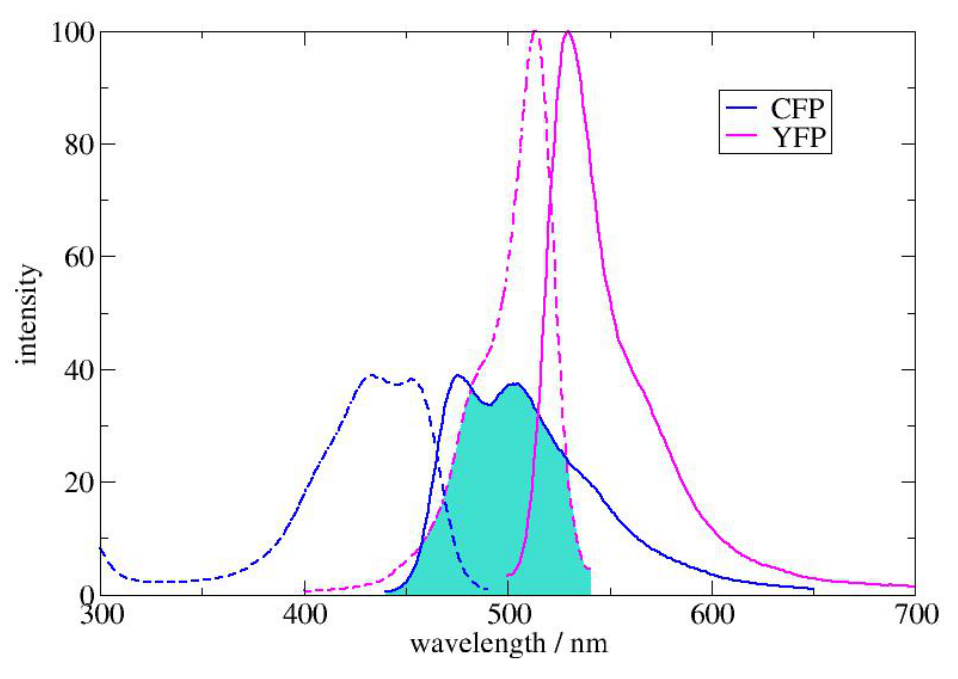
\includegraphics[scale=0.2]{Ueberlappung.png}
    \captionof{figure}{Anregungs- und Emissionsspektrum von CFP und YFP \citep{Anleitung}}
    \label{image:lappung}
\end{center}
Die Vorraussetzung für FRET ist die Überlappung des Emissionsspektrums des Donors und des Absorptionsspektrums des Akzeptors. Diese Vorraussetzung ist bei CFP als Donor und YFP als Akzeptor erfüllt (Durchgezogene blaue Linie zeigt deutliche Überlappung mit gestrichelter pinken Linie in Abb. \ref{image:lappung}). Vertauscht man aber die Rollen von CFP und YFP ist keinen Überlappung mehr gegeben (Durchgezogene pinke Linie schneidet gestrichelte blaue Linie nicht in Abb. \ref{image:lappung} und somit keine Überlappung). Damit ist in diesem Versuch keine FRET-Effekt mit YFP möglich.
\section{Crosstalk-Verunreinigungen}
\label{sec:verunreinigung}
\begin{center}
    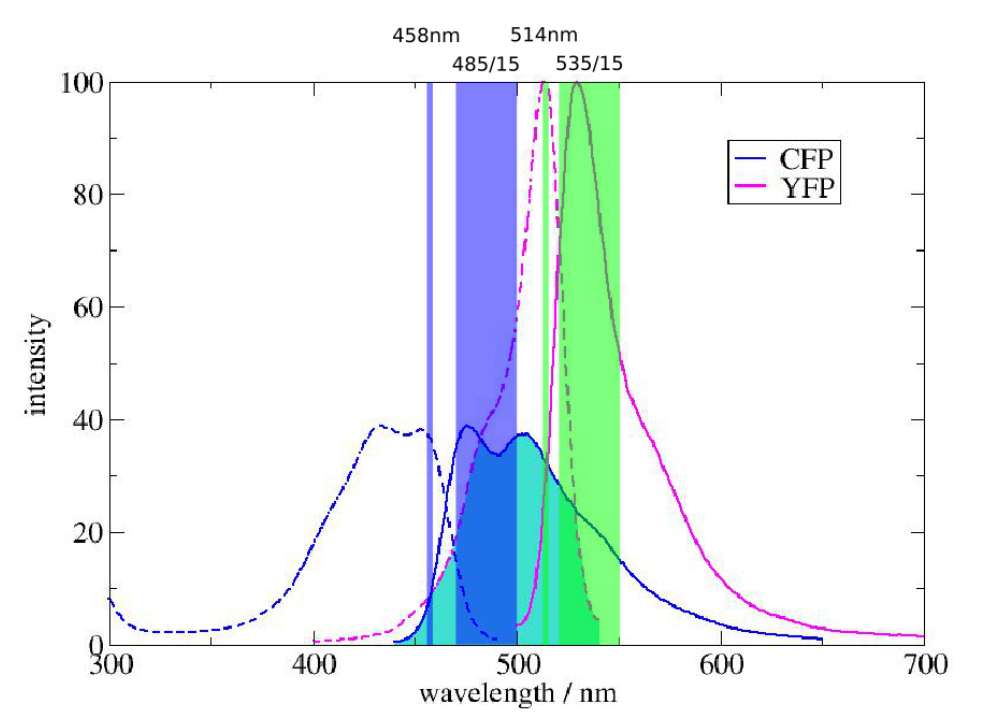
\includegraphics[scale=0.2]{Anregungslinien.png}
    \captionof{figure}{Anregungsbereiche von CFP und YFP \citep{Anleitung}}
    \label{image:anregung}
\end{center}
Die FRET-Intensität kann man nicht direkt messen, da sich der Anregungsbereich der Donors und Akzeptors teilweise überlappen (siehe Abb. \ref{image:anregung}). Somit wird bei einer Anregung des Donors auch der Akzeptor angeregt. Dies führt zu Verunreinigungen in der Messung der Emission des Akzeptors durch die teilweise Anregung. Um diesen Effekt zu korrigieren, misst man die Emission des Donors und die Emission des Akzeptors separat, womit man die Crosstalk Beiträge berechnen kann.
\section{Zeitkorrelierte Einzelphotonenzählung}
Allgemein ist zeitkorrelierte Einzelphotonenzählung (englisch time-correlated single photon counting, TCSPC) eine Technik, um sich zeitlich schnell ändernden Lichtintensitäten zu messen. Diese Messmethode kommt zum Einsatz bei der Messung von Fluoreszenzlebenszeit. Dabei wird die zu untersuchende Probe (Fluorophore) mithilfe von gepulsten Lichtbündel (Laser) angeregt. Die Detektion der Fluoreszenz erfolgt mit einem Photomultiplier, welcher einzelne Photonen registrieren können muss. Die Zeitmessung wird dann durch die Anregung des Laserpuls gestartet und das emittierte Photon stoppt diese. Die Messung wird wiederholt und die einzelnen Photonen werden, mit ihrer entsprechenden Zeit, in ein Histogramm eingetragen. Dieses zeigt einen exponentiellen Abfall der Fluoreszenzintensität nach der Anregung. Der Abfall ergibt sich dann mit der Formel:
\begin{gather}
    N(t) = N_0e^{-\frac{t}{\tau}}~\text{mit}~\frac{1}{\tau} = \sum^m_{i=1} k_i \xrightarrow{n~\text{Proben}} N(t) = \sum_{i=1}^n N_ie^{-\frac{t}{\tau_i}} 
\end{gather} 
Hierbei ist $\tau$ die Lebenszeit aus den $m$ einzelnen Zerfallsraten $k_i$ und $\tau_i$ die Lebenszeit der i-ten Probe mit entsprechender Amplitude $N_i$.\\
Das detektiert Signal hat dann die Form einer Faltung von dem exponentiellen Abfall und einer Gauß-Kurve (entsteht durch die IRF (Impulse Response Function) des Lasers), welches in Abb. \ref{image:abfall} zu sehen ist. Dabei ist der Teil bis zum Peak die IRF und danach der exponentielle Abfall.
\begin{center}
    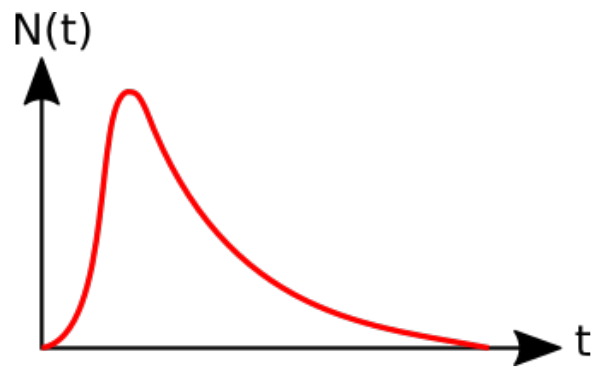
\includegraphics[scale = 0.3]{Abfall.png}
    \captionof{figure}{Verlauf der zeitkorrelierten Einzelphotonenzählung \citep{Anleitung}}
    \label{image:abfall}
\end{center}
\newpage
\subsection*{Störungen}
Bei dieser Messtechnik kann es allerdings zu Störungen kommen, welche das Ergbnis verfälschen.Dazu gehört das thermische Rauschen, wovon beinahe jedes Messgerät betroffen ist. Dies kann durch Kühlung des Messgerätes behoben werden.\\Weitere Störungsfaktoren, sogenannte ’Dark Counting’, sind \textit{Verstärkerrauschen}, \textit{'Afterpulsing'} und \textit{Pile-Up Effekt}.
\begin{itemize}
    \item[(1)] Das \textit{Verstärkerraschen} entsteht durch den angeschlossenen Photomultiplier und lässt sich mit einem Hochpassfilter lösen, da die Amplituden des Rauschens meist geringer sind als die Amplituden der eigentlichen Messung.
    \item[(2)] Beim \textit{'Afterpulsing'} registriert der Detektor nach dem Photonenereignis eine weiteres (fiktives) Ereignis. Behoben kann dies mit der richtigen Wahl des Detektors.
    \item[(3)] Der \textit{Pile-Up Effekt} entsteht durch den Umstand, dass eigentlich nur ein Photon pro Laserpuls mit der Probe wechselwirken kann. Bei mehreren Photonen registriert der Detektor nur das erste Photon, wodurch sich die gemessene Lebensdauer des Photons verringert. Verantwortlich für diesen Effekt ist die Totzeit des Detektors. In dieser Totzeit kann der Detektor kein weiteres Photon detektieren. Verringerung der Laserintensität kann dem Effekt entgegenwirken. \citep{Time}
\end{itemize} 
\newpage
\section{In diesem Versuch verwendete Proben}
\label{sec:proben}
Die verwendeten Proben in diesem Versuch werden mit einem Farbstoff markiert (Proben gehen kovalente Bindung mit Farbstoff-Molekül ein). Bei Anregung emittiert die Probe sichtbare Probe, was den Sachverhalt der Fluoreszenz darstellt.
\begin{center}
    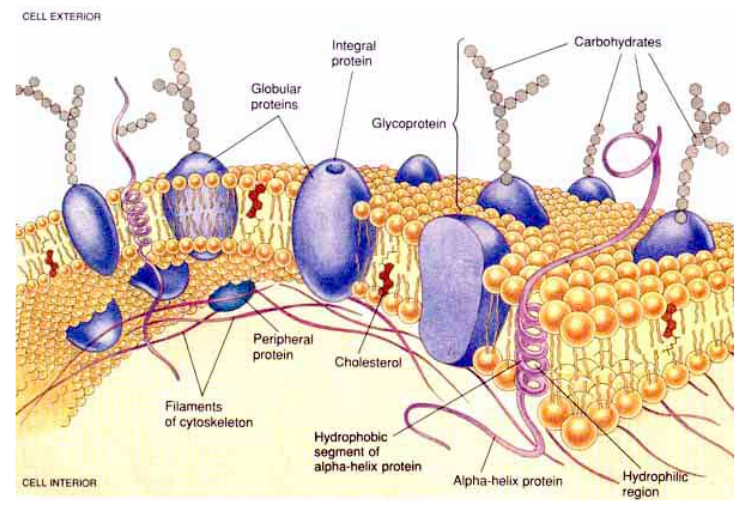
\includegraphics[scale=0.35]{Membran.png}
    \captionof{figure}{Skizze des Plasmamembran \citep{Anleitung}}
    \label{image:membran}
\end{center}
Die genutzte Zelle besitzen ein Plasmamembran, welches aus verschiedenen Lipiden aufgebaut ist (siehe Abb. \ref{image:membran}). Unterhalb der Lipiden sind ca. 30\% Phospholipide und Phosphatidylinositol(4,5)-Bisphosphat (PIP2). PIP2 ist besonders, denn es binden sich im Zellplasma vorhandenen Pleckstrin-Homologiedomäne (PH). In unserem Versuch wird dies verwendet, um CFP und YFP an Proteine mit einer solchen Pleckstrin-Homologiedomäne zu bindet. Durch die hohe Dichte an PIP2 binden sich viele CFP-PH und YFP-PH an das PIP2. Dies hat zur Folge, dass die Distanz zwischen YFP (Akzeptor) und CFP (Donor) gering genug ist, damit die Bedingung für FRET erfüllt ist.
\section{Photobleaching}
\label{sec:bleaching}
Das Photobleaching (dt. Bleichen) ist ein irreversibler Mechanismus, bei dem es zu einem Verlust der Fluoreszenzvon Fluorophoren kommt. Beim Bleaching wird das Fluorophor mit Licht bestrahlt, womit Photonen mit unterschiedlichen Energien auf die Probe treffen. Diese Photonen können vom Fluorophor absorbiert werden und es zu einem Übergang in einen angeregten Zustand (siehe Kapitel \ref{sec:dipolToFRET}). Durch Wechselwirkung zwischen dem angeregten Fluorophor und der Umgebung, kommt es zu einer kovalenten Änderung des Fluorophors, wodurch das Fluorophor seine Fluoreszenz verliert\\ Weiterhin kann man das Fluorophor mithilfe von Quenching (dt. Fluoreszenzlöschung) bleichen, dabei kommt es zu einer Abnahme der Fluoreszenz. Dieser Prozess ist aber zum Gegensatz zum Photobleaching reversibel. \citep{Bleach}
\section{Konfokalmikroskop}
\label{sec:konfokal}
Ein Konfokalmikroskop ist ein spezielles Lichtmikroskop, welches zu jedem Zeitpunkt nur einen Teil der Probe beleuchtet und genau dieser Bruchteil wird dann Stück für Stück abgerastert.
\subsection*{Funtionsweise}
\begin{center}
    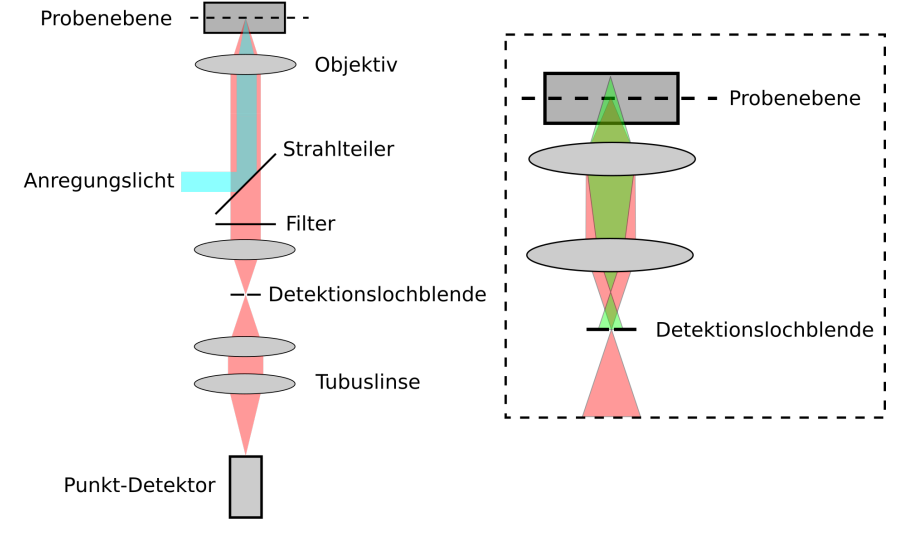
\includegraphics[scale=0.27]{Konfokallinsen.png}
    \captionof{figure}{Prinzipieller Aufbau eines Konfokalmikroskop \citep{Anleitung}}
    \label{image:konfokal}
\end{center}
In Abb. \ref{image:konfokal} wird der prinzipielle Aufbau eines Konfokalmikroskop gezeigt. Dabei wird der Anregungsstrahl (blau in \ref{image:konfokal}) durch einen Strahlenteiler reflektiert und durch eine Linse gebündelt mit dem Brennpunkt auf der Probe. Von der Probe wird dann der sogenannte Detektionsstrahl (rot in \ref{image:konfokal}) ausgesendet. Dieser Strahl wird durch die oberste Linse parallelisiert und trifft auf den Strahlenteiler, der den Strahl transmittieren lässt. Nach dem Strahlenteiler kann ein Filter eingebaut werden, welcher die störenden Wellenlängen herausfiltert. Nach dem Filter befindet sich eine weitere Linse und die Detektionslochblende, welche das Detektionsvolumen auf einen kleinen Bereich einschränkt. Dies bedeutet das Strahlen aus einem hinteren Bereich der Probe nicht zum Detektor gelangen. Nach der Blende trifft der Detektionsstrahl auf die erste Tubuslinse. Diese parallelisiert den Strahl erneut und die zweite Tubuslinse fokussiert ihn auf den Punkt-Detektor. Der Punkt-Detektor registriert dann die einzelnen Photonen.
\subsection*{Vor und Nachteile}
\begin{itemize}
    \item[\textcolor{green}{\textbf{+}}] Unerwünschtes Hintergrundrauschen (z.B. Streulicht) reduzierbar auf ein Minimum und bessere Auflösung zum Vergleich zu konventionellen Mikroskopen wegen der Detektionslochblende
    \item[\textcolor{red}{\textbf{-}}] Detektionslochblende kann Beugungserscheinungen verursachen, was die Auflösung begrenzt
\end{itemize}
Als Alternative zum Konfokalmikroskop kann das Laser-Scanning-Microscope verwendet werden, welches ohne die Detektionslochblende auskommt und eine höhere Auflösung besitzt.

    % 3.Kapitel Protocol
    % 3. Protocol

\chapter{Protocol}
\label{chap:protocol}

\section*{Adjustment for measurement}
We adjust the test setup after instruction of the supervisor with the adjusting tip. For that we make sure to take two points for two mirrors that are as far as possible away from the specific mirror.

\section*{Chanels}

\begin{tabular}[]{c|c|l}
    Input & Output & Description\\
    \hline
    ai0 & RF Output & balance of reference beam and measurement beam\\
    ai1 & Monitor + & measurement beam\\
    ai3 & Monitor - & reference beam\\
    ai4 & PD2 Output & signal of fabry-pérot-interferometer\\
\end{tabular}\\

For our files we have taken the name: \textit{MesN\_TempY\_ZPeaks} there $N$ is number of the measurement/id and $Y$ is the temperature \SI{24}{\celsius}, \SI{38}{\celsius}, \SI{56,2}{\celsius} without the unit and $Z$ is the number to identify the peak with the values all, 1, 2, 3, 4 which is number from left to right.
To every measurement we save a .dat-file and a .bmp-file on our usb-stick.
We also used always the act-value and not the set-value for measurement.

\section*{Measurement}
\begin{itemize}
    \item \textbf{Temperature: \SI{24}{\celsius}} \\ 
    Filename: \textit{date+time\_group11\_MesN\_Temp24\_ZPeak.dat and .bmp}\\ $N$ from 1 to 5, act-value: \SI{24}{\celsius}
    \item \textbf{Temperature: \SI{38}{\celsius}} \\ 
    Filename: \textit{date+time\_group11\_MesN\_Temp38\_ZPeak.dat and .bmp}\\ $N$ from 6 to 10, act-value: \SI{40}{\celsius}
    \item \textbf{Temperature: \SI{56,2}{\celsius}} \\ 
    Filename: \textit{date+time\_group11\_MesN\_Temp38\_ZPeak.dat and .bmp}\\ $N$ from 11 to 15, act-value: \SI{60}{\celsius}
    \item \textbf{Distance fabry-pérot-interferometer:} \SI{72,5}{\centi\metre}+\SI{36}{\centi\metre}+\SI{43}{\centi\metre}=\SI{151,5}{\centi\metre}\\ measured with tape measure
\end{itemize}

\begin{center}
    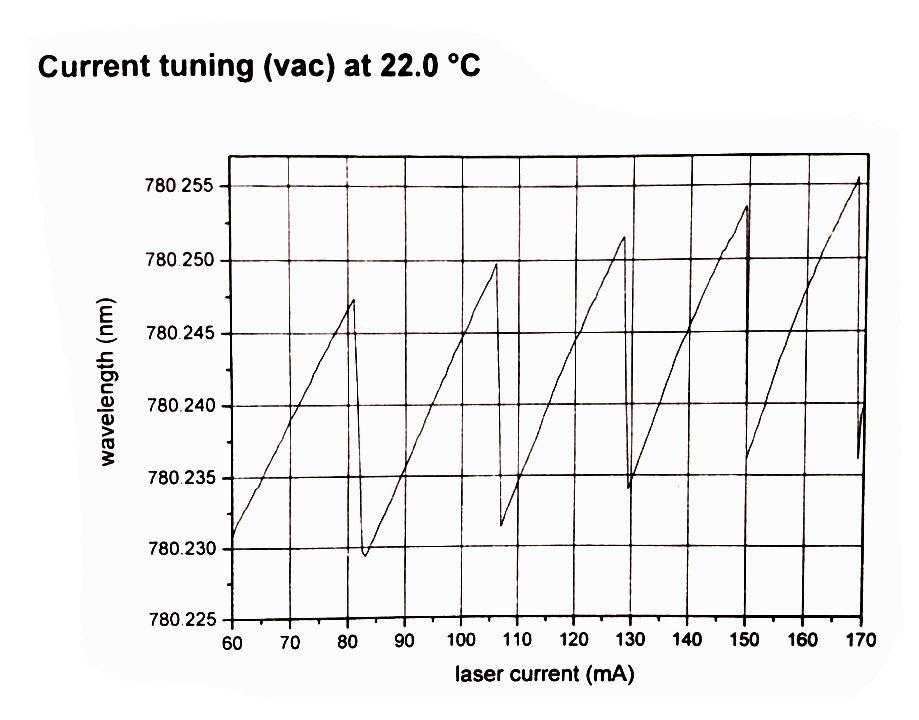
\includegraphics[scale = 0.4]{currentTuning.jpg}
    \captionof{figure}{Currunt Tuning at \SI{22}{\celsius} from laser instructions}
    \label{image:currentTuning}
\end{center}

    % 4.Kapitel Evaluation
    % 4. Evaluation

\chapter{Evaluation}
\label{chap:eval}
We have chosen to take the measured data for \SI{24}{\celsius}, because the reference beam and the sample beam have had the best alignment. It seems also in this data the observation of the height of the lamb dips and the width of the lines would be much easier as in the other temperatures.

% Text

% Part 1

\section{Freeing Absorption Spectrum from Trend and identify Lines}
\label{sec:freeing}
Now we want to free the spectrum from any trend for that the fit a linear function on the spectrum of the reference beam and subtract the fit from the sample beam and reference beam. It is worth mentioning that we have moved the reference beam spectrum down to the niveau of the sample beam spectrum and after that we fitted the linear function. In fig. \ref{image:trends} we can see the absorption spectrum with trends and the linear fit and in fig. \ref{image:trendless} the spectrum without trends. The fit is managed with the function polyfit of the numpy-module in python. We did also cut the data so that we can clearly see the four peaks without any jumps in mode.
\begin{center}
    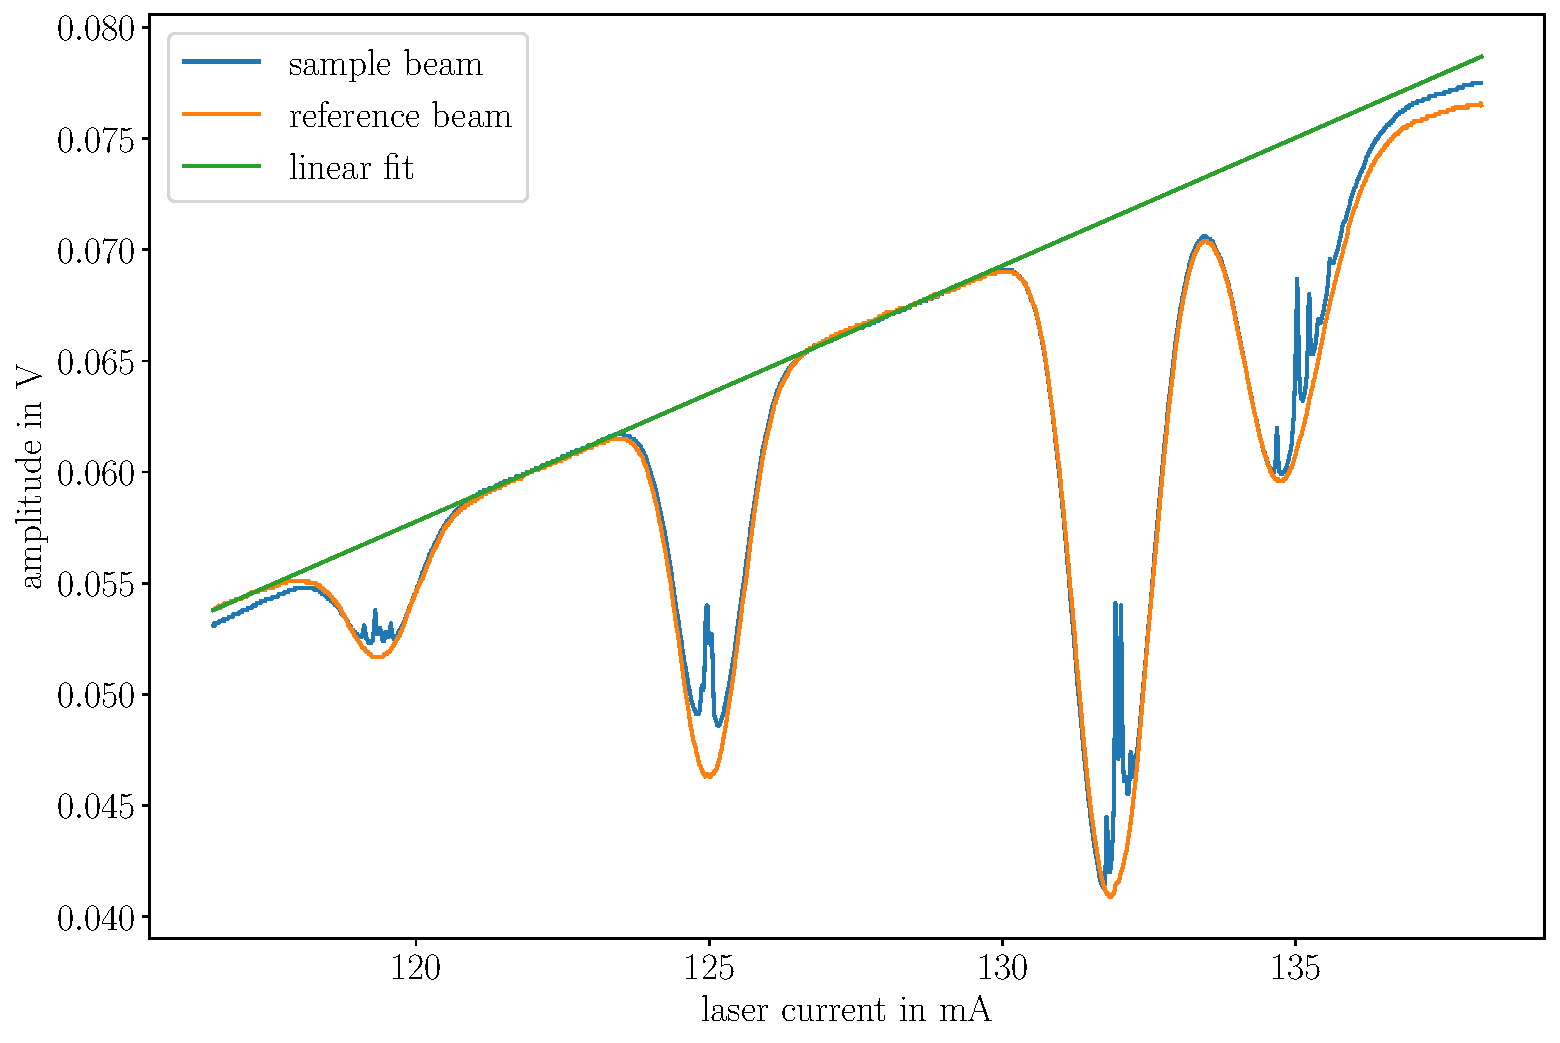
\includegraphics[scale=0.47]{Aufg-1/trend24.pdf}
    \captionof{figure}{absorption spectrum with trends}
    \label{image:trends}
\end{center}
\begin{center}
    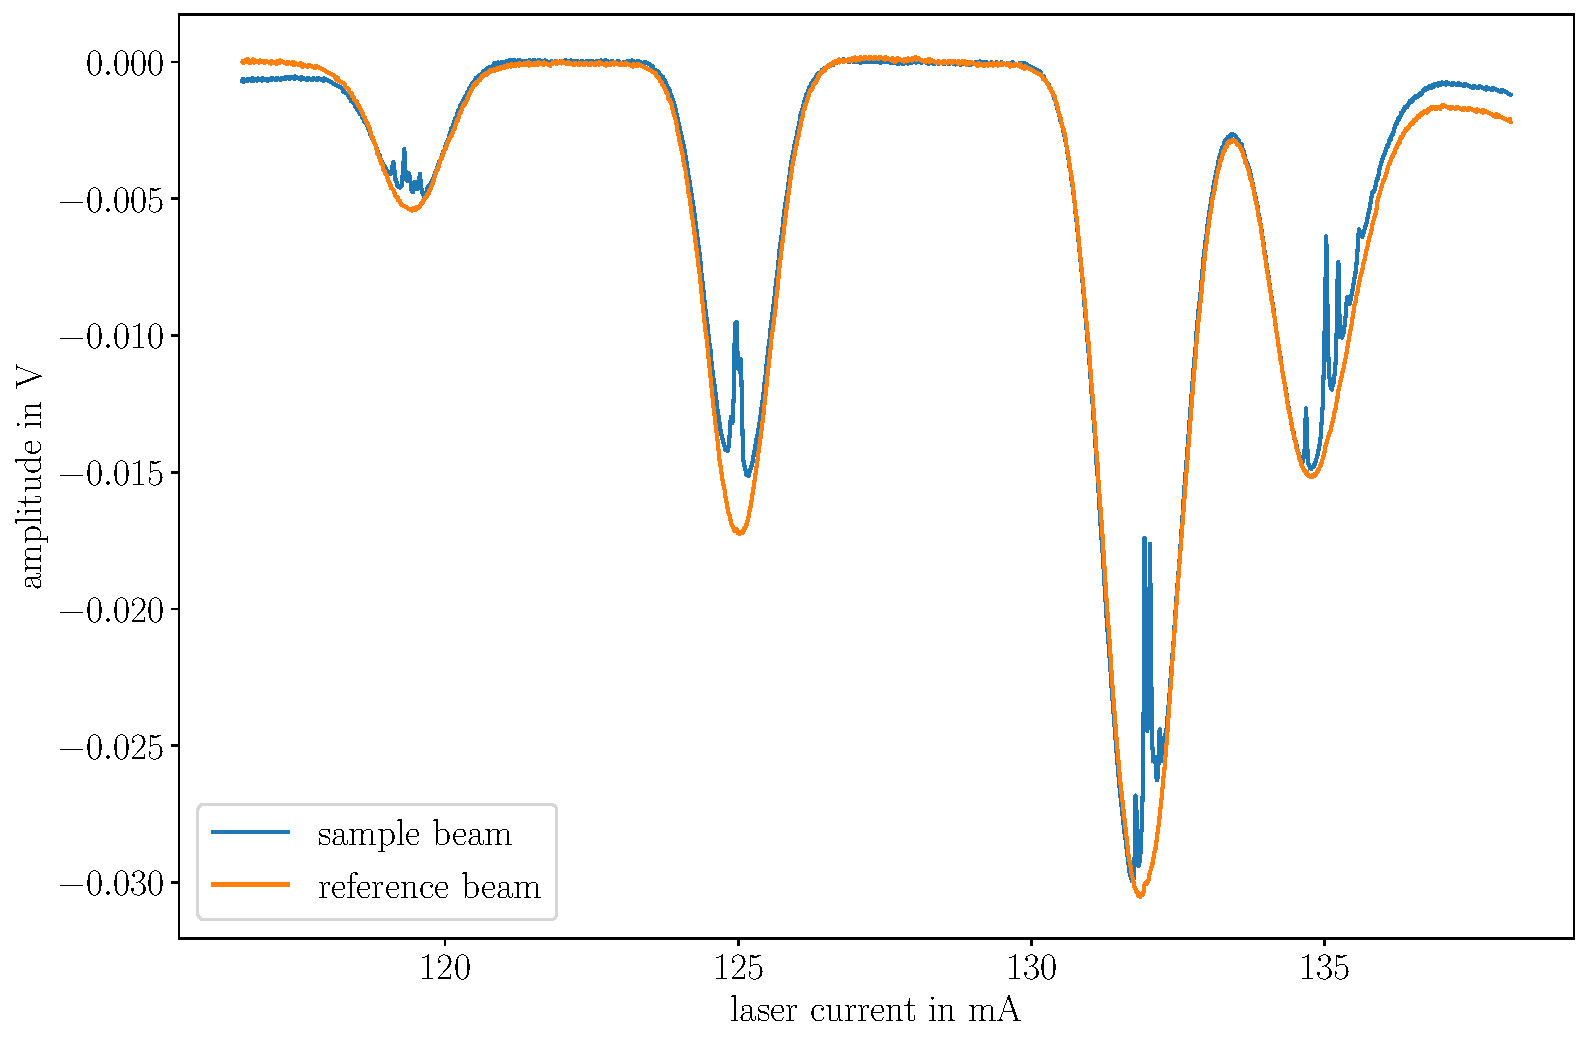
\includegraphics[scale=0.47]{Aufg-1/trendless24.pdf}
    \captionof{figure}{absorption Spectrum without trends}
    \label{image:trendless}
\end{center}
We applied the same procedure on the data of the fabry-pérot and see clear in fig. \ref{image:allTrendless} that the signal is not very stable, but this is not from interest for the upcoming evaluation because we need only the distance between to peaks.
\begin{center}
    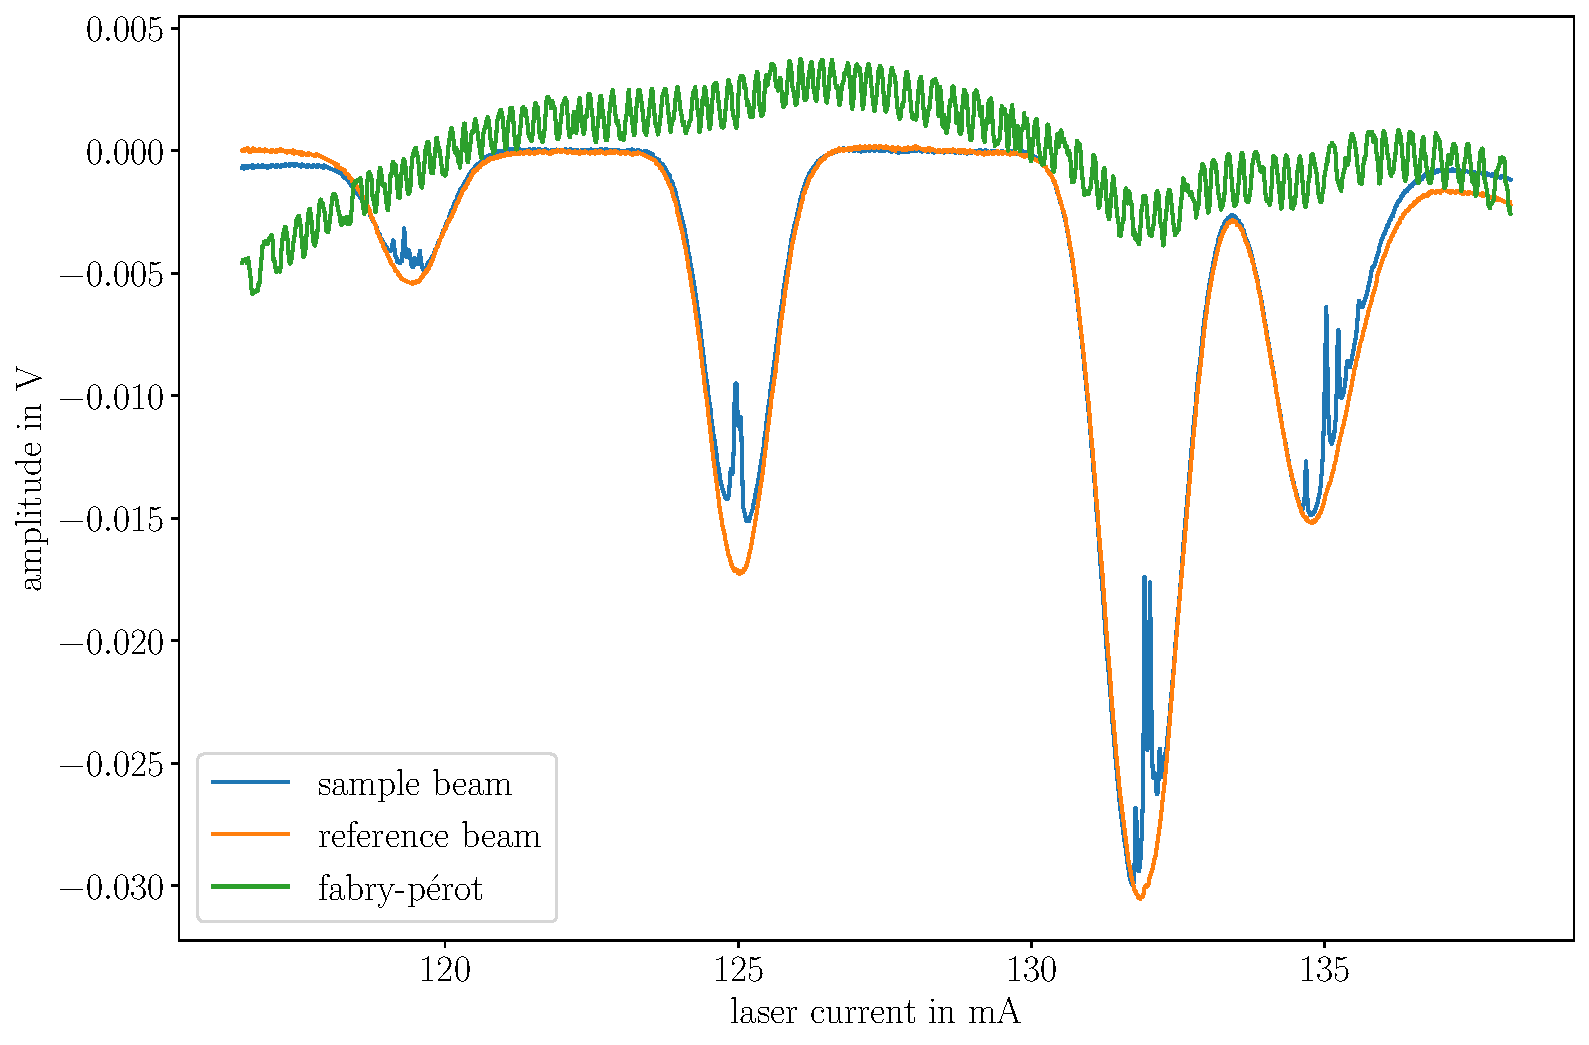
\includegraphics[scale=0.47]{Aufg-1/alltrendless24.pdf}
    \captionof{figure}{absorption spectrum without trends all channels}
    \label{image:allTrendless}
\end{center}
\subsection*{Identfication considering intensity and order}
To identify the lines of the spectrum we used the current wavelength curve (look fig. \ref{image:currentTuning}) to convert the laser current to the wavelength. To do this we convert the fig. \ref{image:currentTuning} into a csv-file using python. For that we measured roughly the points of the peaks from 105 mA to 150 mA (because that is the area of interest) and calculated a basic linear function of the form $y=mx +t$ between them (look fig. \ref{image:currentTuningCut}). Then we obtain three separate linear functions that can transform our data in the corresponding wavelength in the specific area of the current wavelength curve.
\begin{center}
    \begin{tabular}{c | c c c c}
        {} & 1 & 2 & 3 & 4 \\
        \hline
        laser current/mA & 107.0 & 128.5 & 129.5 & 149.5\\
        wavelength/nm & 780.23125 & 780.25125 & 780.234 & 780.2535\\
    \end{tabular}
    \captionof{table}{point used for recreating current wavelength curve}
    \begin{tabular}{c | r r }
        area & m/$\frac{\text{nm}}{\text{mA}}$ & t/nm\\
        \hline
        $1 \rightarrow 2$ & 0.00093  & 780.132 \\
        $2 \rightarrow 3$ & -0.01725 & 782.468 \\
        $3 \rightarrow 4$ & 0.00097  & 780.108 \\
    \end{tabular}
    \captionof{table}{linear functions of the current wavelength curve}
\end{center}
\begin{center}
    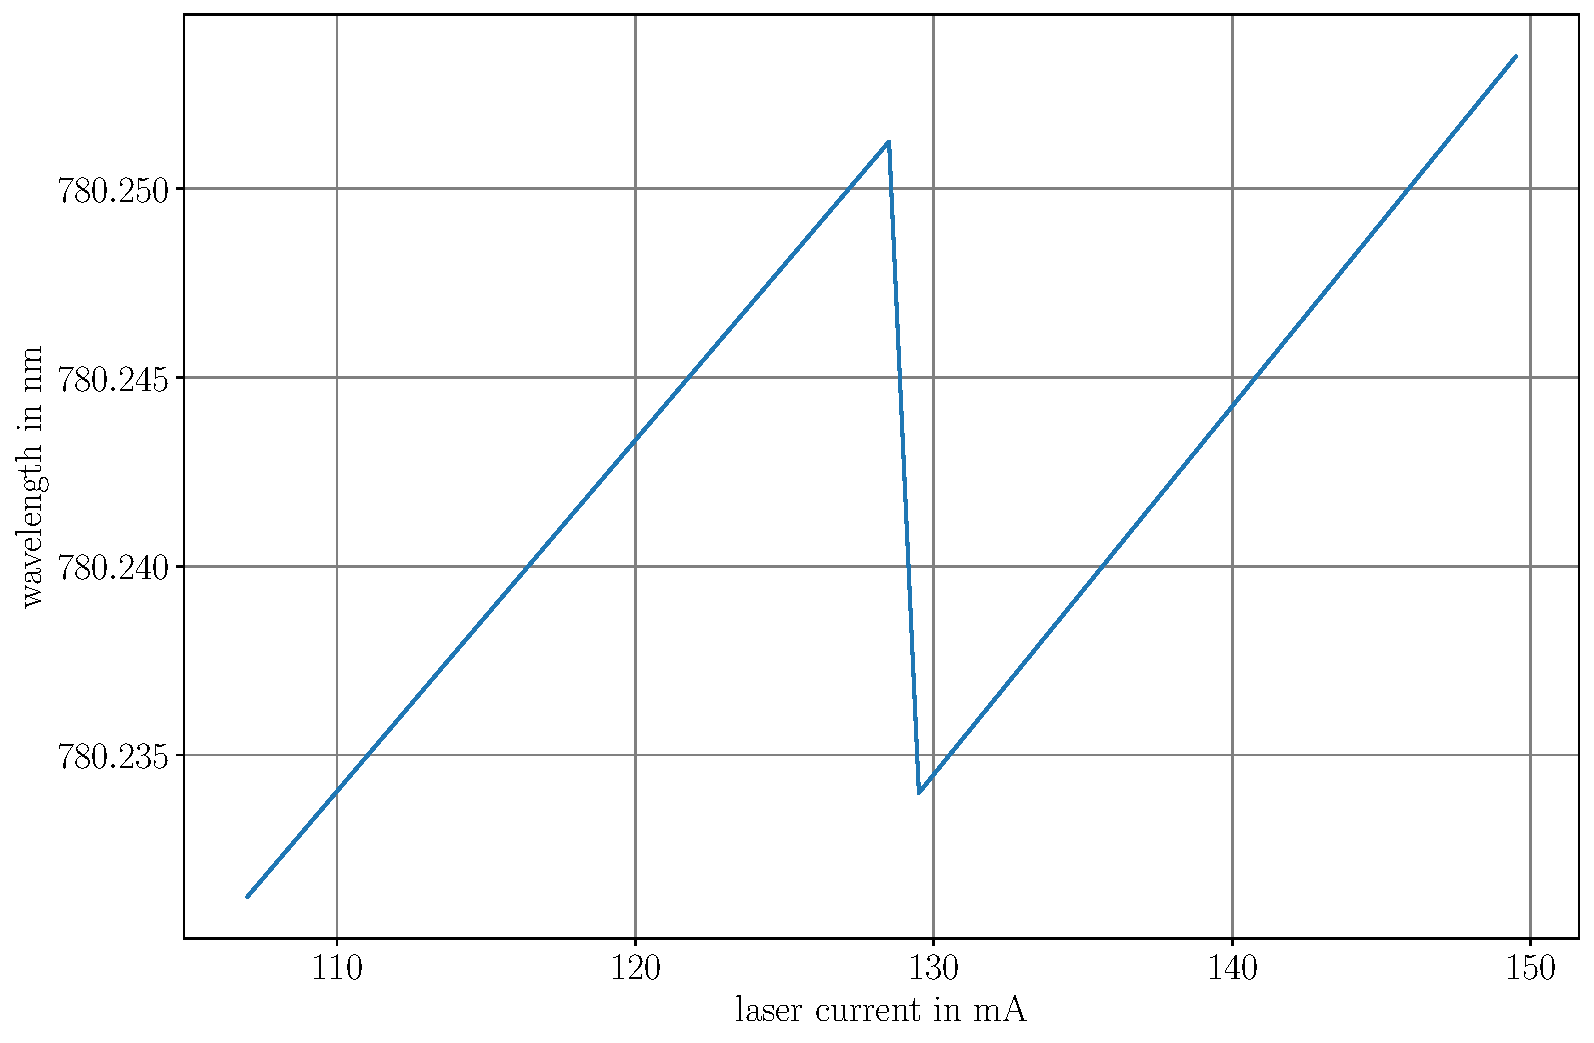
\includegraphics[scale=0.45]{Aufg-1/currentTuning.pdf}
    \captionof{figure}{cut current wavelength curve from 105 mA to 150 mA using python}
    \label{image:currentTuningCut}
\end{center}
From the csv-file we can easily find our value for the peaks of the reference beam and convert them into the corresponding wavelength. Then we compared the measured wavelength with the literature \citep{RDL85,RDL87} there $F$ are the quantum number of the $5^2S_{1/2}$-state.
\begin{center}
    \begin{tabular}{c | c | c c c | c c }
        \makecell{peak\\order} & \makecell{laser\\current/mA} & \makecell{wavelength\\measured/nm} & \makecell{wavelength\\literature/nm} & deviation/nm & isotope & $F$ \\
        \hline
        1 & 119.4429 & 780.243 & 780.233 & 0.010 & $^{87}Rb$ & 1 \\
        2 & 125.0267 & 780.248 & 780.238 & 0.010 & $^{85}Rb$ & 2 \\
        3 & 131.8581 & 780.236 & 780.244 & 0.008 & $^{85}Rb$ & 3 \\
        4 & 134.7829 & 780.239 & 780.246 & 0.007 & $^{87}Rb$ & 2 \\       
    \end{tabular}
    \captionof{table}{identification by intensity and order}
    \label{tab:identify}
\end{center}
Because $^{85}Rb$ have to be isotope with the highest occurrence we can clearly identify the highest peaks of the absorption spectrum as the one of $^{85}Rb$. In addition to that we can conclude that the measured data have some kind of bias, roughly 0.010 nm, in each area of the current wavelength curve of the laser.
\section{Distance between Energy Levels}
\label{sec:distance}
\subsection*{Current Wavelength Curve}
As mentioned in chapter \ref{sec:freeing} we already have transformed all data into the wavelength using the current wavelength curve. Because of that the order of the identified peaks from table \ref{tab:identify} has changed to 3 (${85}^Rb$, $F=3$), 4 (${87}^Rb$, $F=2$), 1 (${87}^Rb$, $F=1$), 2 (${85}^Rb$, $F=2$). The next step is to transform the wavelength into the frequency using the formula $\nu=\frac{c}{\lambda}$, where $c$ is the speed of light in vacuum. The result can be seen in fig. \ref{image:fequency} where the new order of the peaks is 3, 4, 1, 2.
\begin{center}
    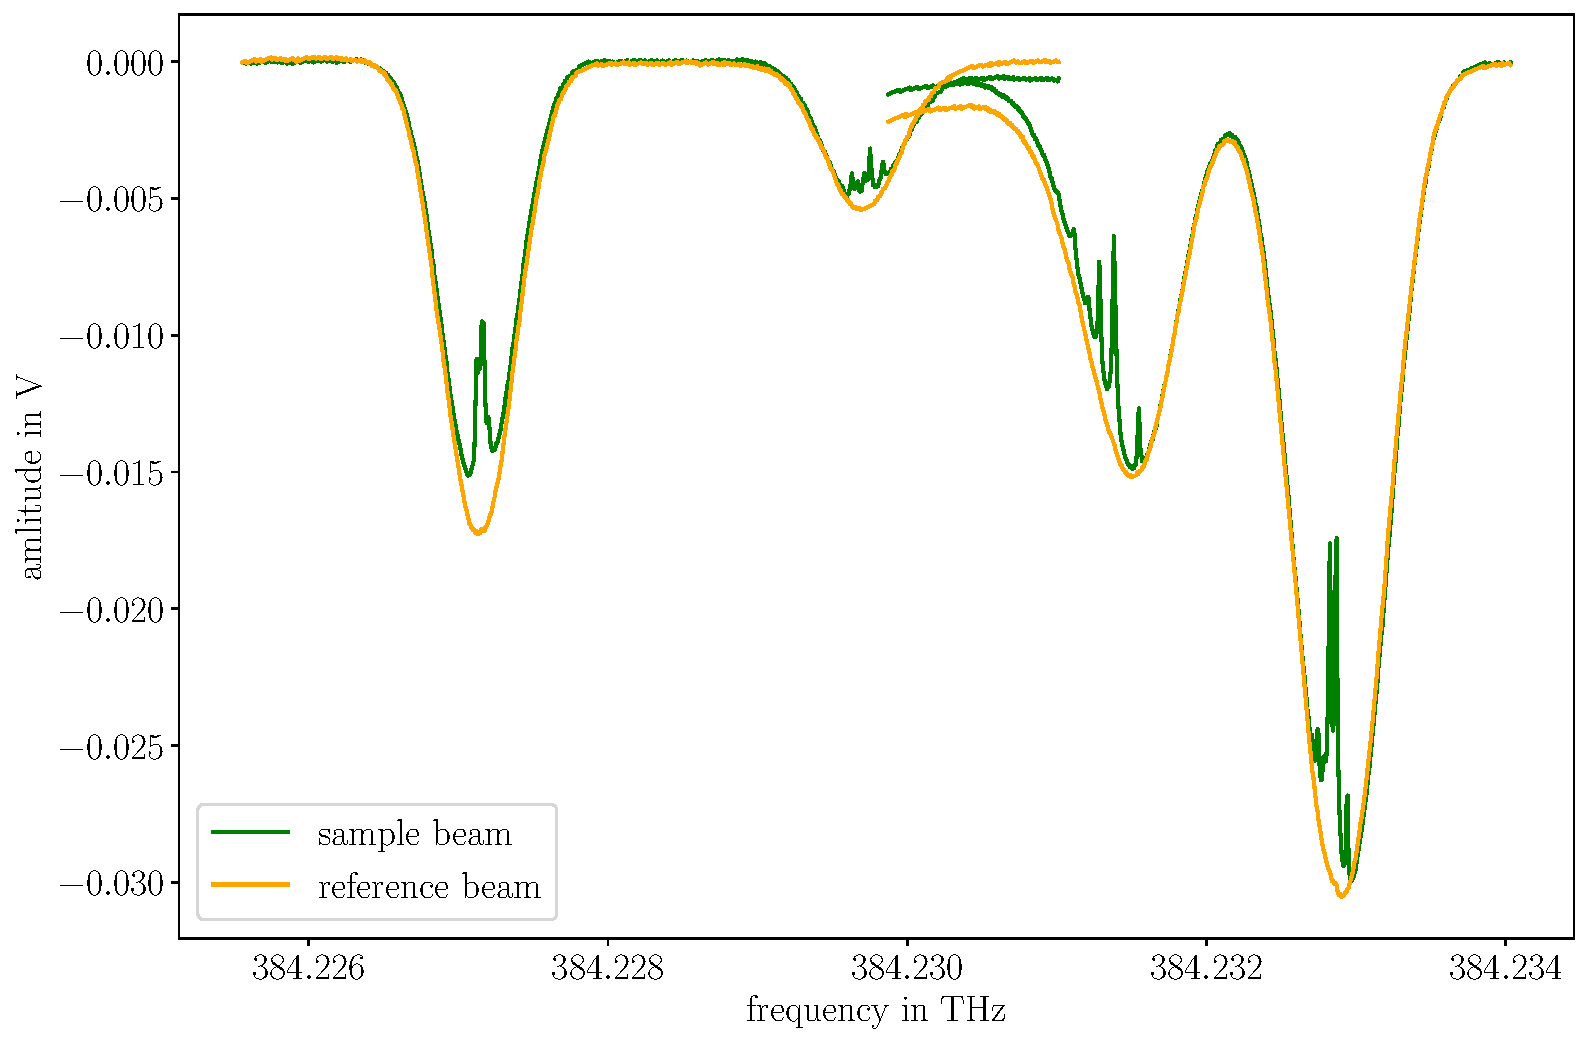
\includegraphics[scale=0.47]{Aufg-2/frequencyallPeakTemp24.pdf}
    \captionof{figure}{absorption spectrum after transformation to \textbf{frequency}}
    \label{image:fequency}
\end{center}
One can also see the occurrence of overlapping in fig. \ref{image:fequency} that is caused by the transformation from the laser current to the wavelength. It is possible to erase the overlapping lines from the data but for this evaluation it is necessary.
By using the same method as in chapter \ref{sec:freeing} to identify the peaks we obtain distance as followed:
\begin{center}
    \begin{tabular}{c | c}
        peak area & $d_{current}$/THz\\
        \hline
        $2 \rightarrow 1$ & 0.00256\\
        $1 \rightarrow 4$ & 0.00181\\
        $4 \rightarrow 3$ & 0.00140\\
    \end{tabular}
    \captionof{table}{distances between the energy levels using current wavelength curve}
    \label{tab:currentMethode}
\end{center}
\subsection*{Fabry-Pérot Interferometer}
To calculate the distance of the energy level we start using the function of the Fabry-Pérot interferometer and insert the measured length $d$:
\begin{gather}
    \Delta\omega_{FSR} = \frac{c}{2nd} \overset{n=1}{=} \frac{c}{2d} \overset{d=\SI{1.515}{\metre}}{=} \SI{98.9}{\mega\hertz} 
\end{gather}
In the trendfree line of the interferometer we can count from 117.0455 mA to 137.6816 mA an amount of 97 maxima peaks. For each peak we get a current value that we convert into relative frequency $\Delta\omega_{FSR}$ starting with the value 0 for the first peak. This gives us the figure \ref{image:relfequency}.
\begin{center}
    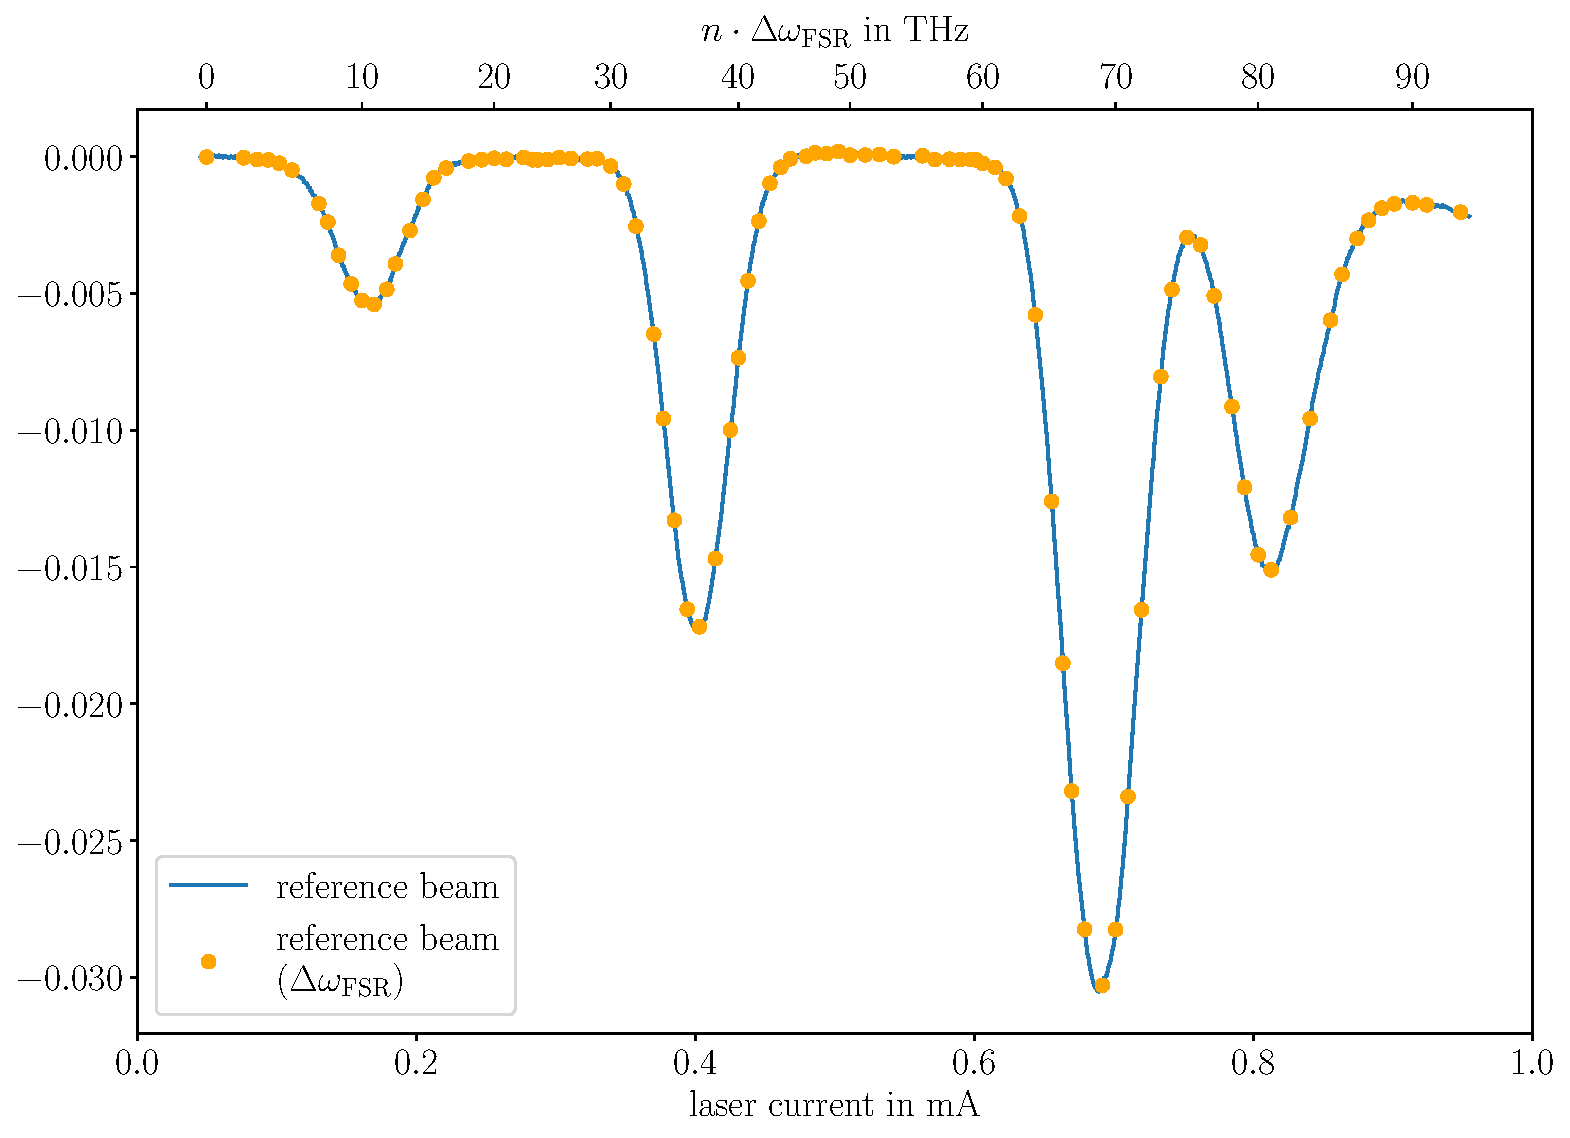
\includegraphics[scale = 0.45]{Aufg-2/relfrequencyallPeakTemp24.pdf}
    \captionof{figure}{absorption spectrum after transformation to \textbf{relative frequency}}
    \label{image:relfequency}
\end{center}
In the upcoming figures we decided to abstain from including the relative frequency transformed data for clearness. 
\newpage
In following we count the amount of fabry-pérot interferometer peaks between each peak of the absorption spectrum and multiply that with $\Delta\omega_{FSR}$. That gives us in comparsion with the calculated data from table \ref{tab:currentMethode}:
\begin{center}
    \begin{tabular}{c | c c c}
        peak area & difference/mA & $d_{interferometer}$/THz & $d_{current}$/THz\\
        \hline
        $1 \rightarrow 2$ & 5.5838 & $26\cdot\Delta\omega_{FSR} = 0.00257$ & 0.00256\\
        $2 \rightarrow 3$ & 6.8314 & $32\cdot\Delta\omega_{FSR} = 0.00316$ &   ---  \\
        $3 \rightarrow 4$ & 2.9248 & $12\cdot\Delta\omega_{FSR} = 0.00119$ & 0.00140\\
    \end{tabular}
    \captionof{table}{distance between the energy levels using Fabry-Pérot interferometer and comparison to usage of current wavelength curve}
    \label{tab:interferometerMethode}
\end{center} 
In table \ref{tab:interferometerMethode} we can clearly see that both methods are equal in evaluation.
\newpage

%\begin{gather}
%    \frac{97\cdot \Delta\omega_{FSR}}{\SI{137.6816}{\milli\ampere}-\SI{117.0455}{\milli\ampere}} = 0.465\frac{\si{\giga\hertz}}{\si{\milli\ampere}}
%\end{gather}
%This means that 1 mA correspond to \SI{0.465}{\giga\hertz}.

%In following we use the table \ref{tab:identify} from chapter \ref{sec:freeing} for the information of the current for each peak and take the difference of them. That gives us in comparsion with the calculated data from table \ref{tab:currentMethode}:
%\begin{center}
%    \begin{tabular}{c | c c c}
%        peak area & difference/mA & $d_{interferometer}$/THz & $d_{current}$/THz\\
%        \hline
%        $1 \rightarrow 2$ & 5.5838 & 0.00260 & 0.00256\\
%        $2 \rightarrow 3$ & 6.8314 & 0.00318 &   ---  \\
%        $3 \rightarrow 4$ & 2.9248 & 0.00136 & 0.00140\\
%    \end{tabular}
%    \captionof{table}{distance between the energy levels using Fabry-Pérot interferometer and comparison to usage of current wavelength curve}
%    \label{tab:interferometerMethode}
%\end{center} 
\section{The real ratio of the rubidium isotopes}
\label{sec:ratio}
Now we calculate the ratio of each isotope by identifying the area under every peak. For that we are fitting the gaussian distribution for each peak of our data for the reference beam absorption spectrum. We take the current axis because for the ratio it does not matter which axis we use. Furthermore, we use the data that is freed from any trends (look fig. \ref{image:trendless}).Then the fitting function has the form of:
\begin{gather}
    y = a\cdot\exp(-\left(\frac{(x-b)}{\sqrt{2}c}\right)^2)
    \label{eq:gaussFit}
\end{gather}
$b$ is here the x-value of each peak that we have already obtained in table \ref{tab:identify}. We get with the curve_fit of scipy.optimize package from python:
\begin{center}
    \begin{tabular}{c | c c c}
        peak & a/V & b/mA & c/mA\\
        \hline
        1 &  -0.00539 & 119.4429 & 0.57669\\
        2 &  -0.01742 & 125.0267 & 0.52976\\
        3 &  -0.03085 & 131.8581 & 0.62443\\
        4 &  -0.01462 & 134.7829 & 0.74425\\
    \end{tabular}
    \captionof{table}{fitting data for each peak}
\end{center}
In figure \ref{image:gaussFit} is shown how each gaussian fit looks for each peak.\\
With the parameter we calculated above we are now able to determine the area under each curve of each peak with the following relation:
\begin{gather}
    \int^{\infty}_{-\infty}\exp(-k(x-\mu)^2)\,dx = \sqrt{\frac{\pi}{k}} \xrightarrow{\mu = b,~k = \frac{1}{2c^2}}\int^{\infty}_{-\infty}a\cdot\exp(-\left(\frac{(x-b)}{\sqrt{2}c}\right)^2) = a \sqrt{2\pi c^2}
\end{gather}
This expression gives us then the area as follows:
\begin{center}
    \begin{tabular}{c | c | c}
        peak & isotope & area/$1\cdot 10^{-6}$ W\\
        \hline
        1 & $^{87}Rb$ &  -7.79 \\
        2 & $^{85}Rb$ & -23.13 \\
        3 & $^{85}Rb$ & -48.29 \\
        4 & $^{87}Rb$ & -27.27 \\
    \end{tabular}
    \captionof{table}{area under the curve of each peak}
\end{center}
The area under the peaks is proportional to the amount of atoms of each isotope in the gas what gives us:
\begin{gather}
    ^{85}Rb = \frac{23.13+48.29}{7.79+23.13+48.29+27.27} = 0.671 \Rightarrow  {^{87}Rb} = 0.329
\end{gather}
Meaning that in our probe there is \SI{67.1}{\percent} $^{85}Rb$ and \SI{32.9}{\percent} $^{87}Rb$ which compared to the literature \citep{RDL85,RDL87} (\SI{72.2}{\percent} $^{85}Rb$ and \SI{27.8}{\percent} $^{87}Rb$) shows that the assumption from chapter \ref{sec:freeing} to take the intensity into account was correct.
\begin{center}
    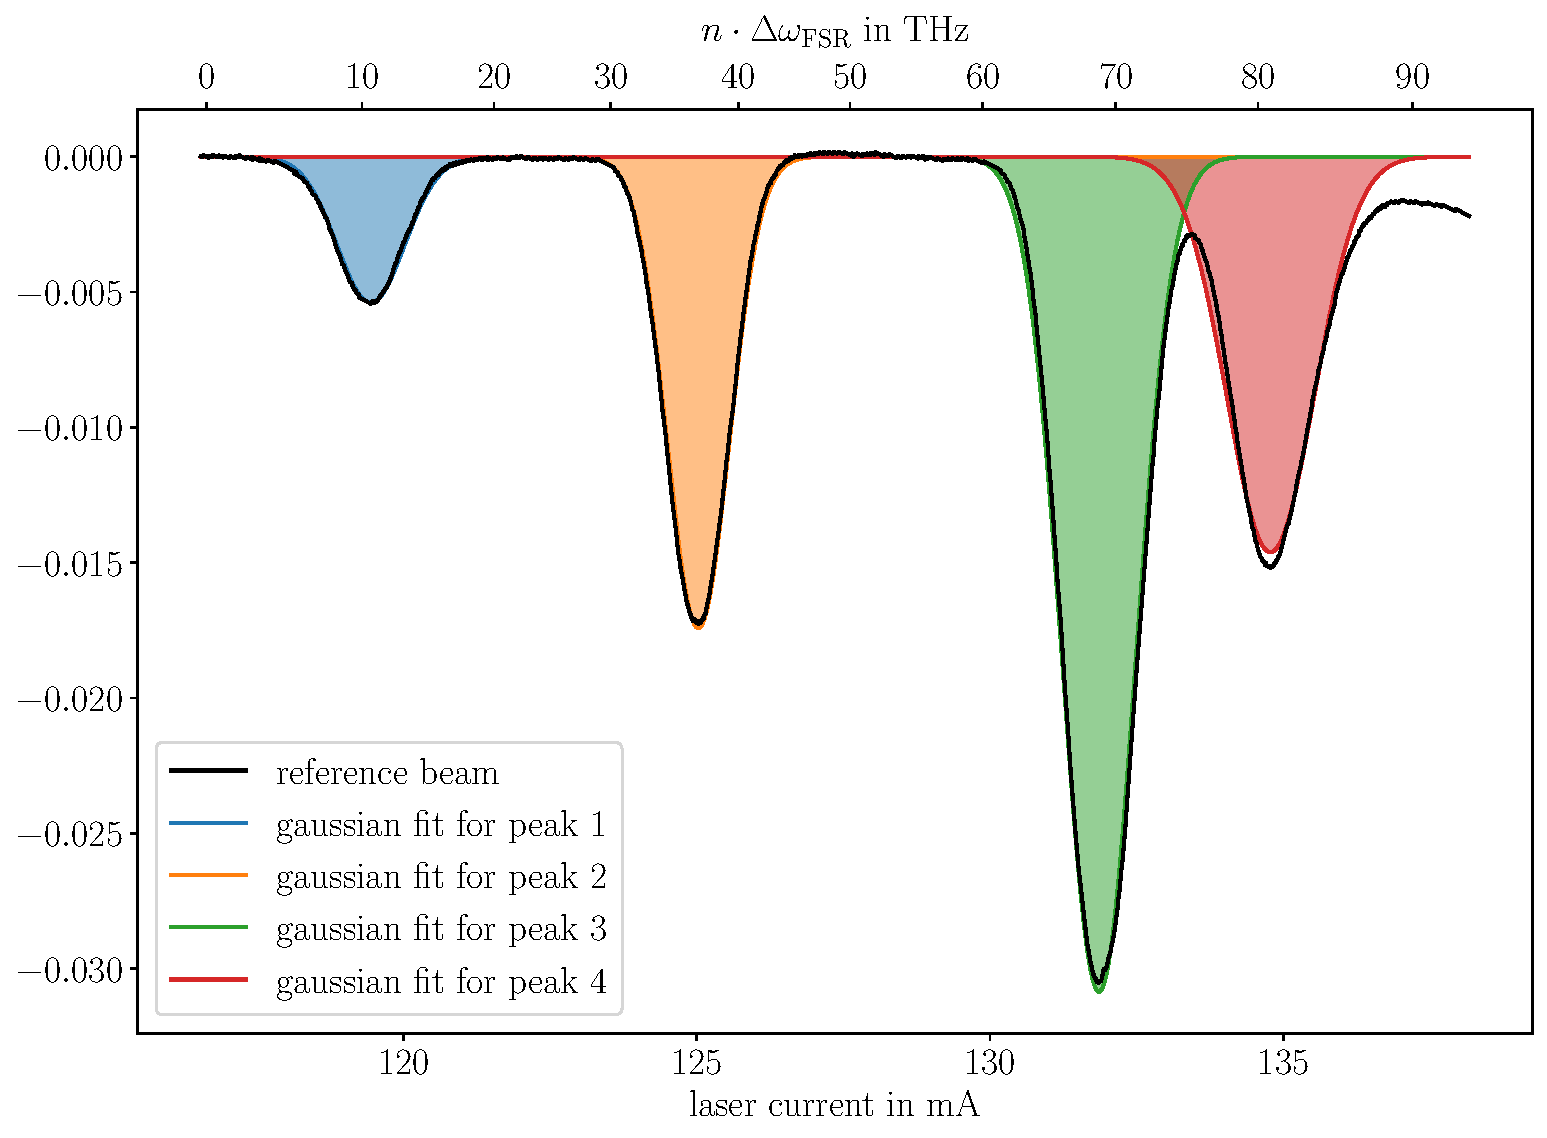
\includegraphics[scale=0.72, angle = 90]{Aufg-3/gaussFit.pdf}
    \captionof{figure}{gaussian fit for each Peak of the reference beam spectrum}
    \label{image:gaussFit}
\end{center}
\section{Hyperfine Dips}
\label{sec:hyperfine}
Firstly we want to show all absorption dips separately starting with peak 1 and ending with peak 4.
\begin{center}
    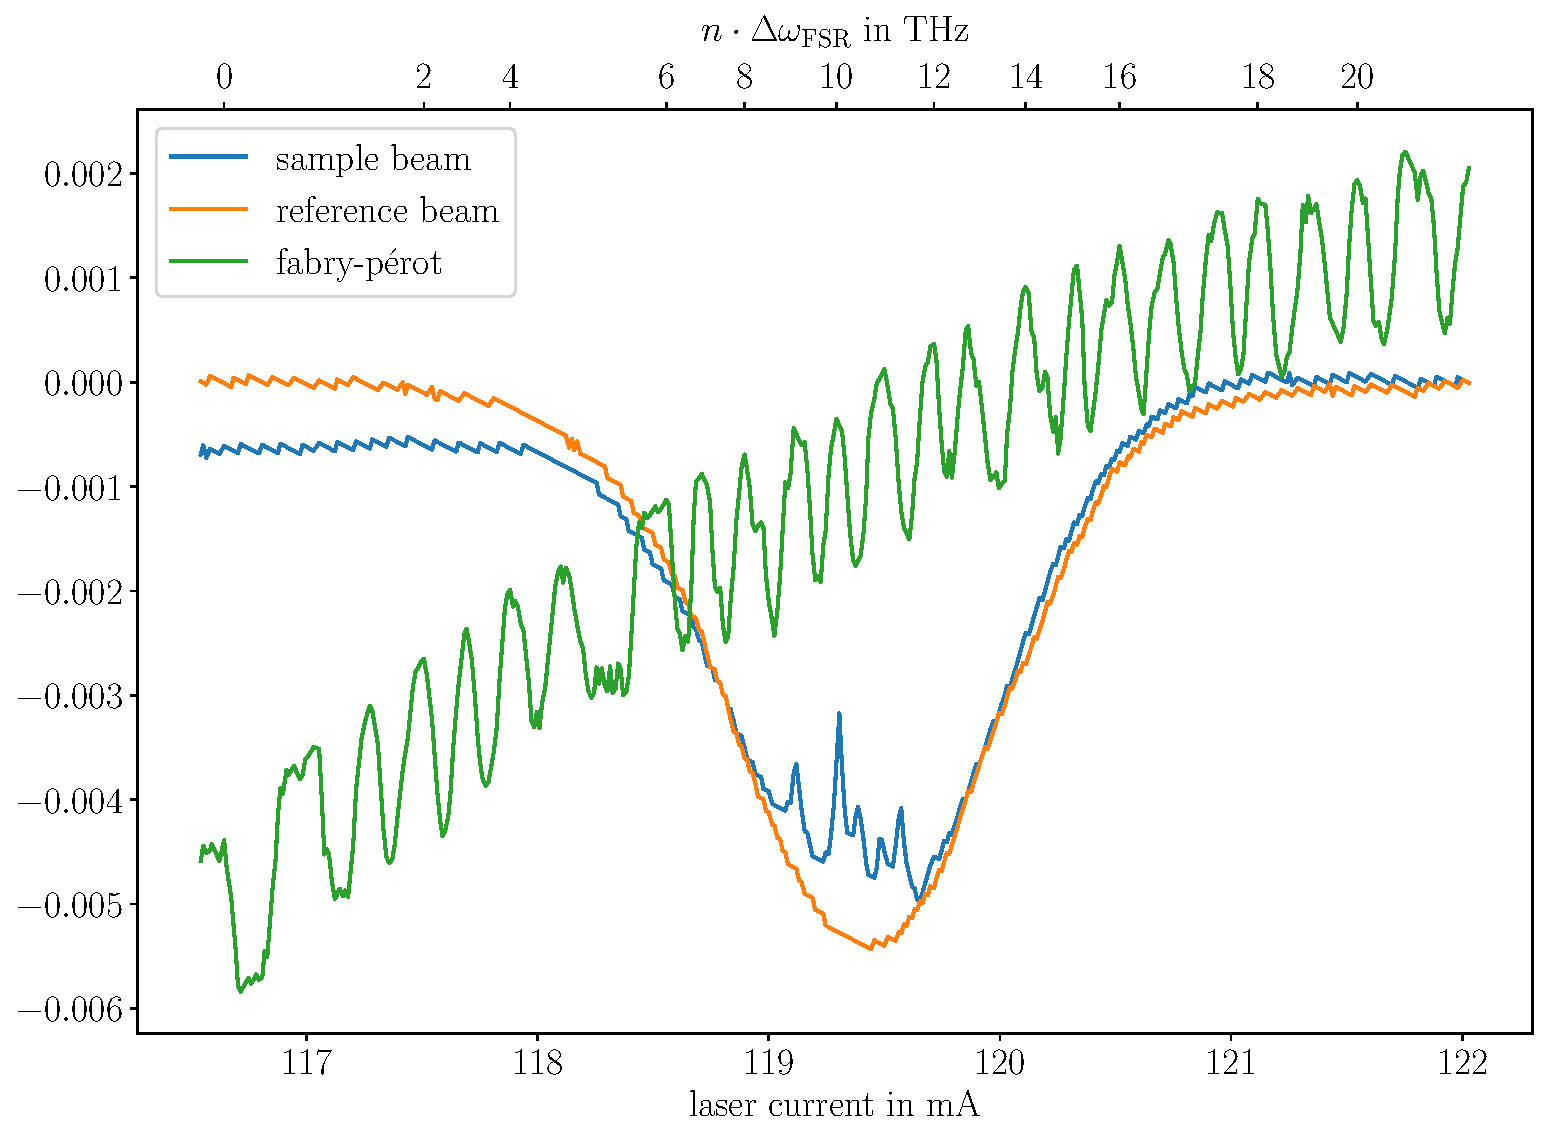
\includegraphics[scale=0.45]{Aufg-4/hyperfine1.pdf}
    \captionof{figure}{absorption spectrum of peak number 1}
    \label{image:peak1}
\end{center}
\begin{center}
    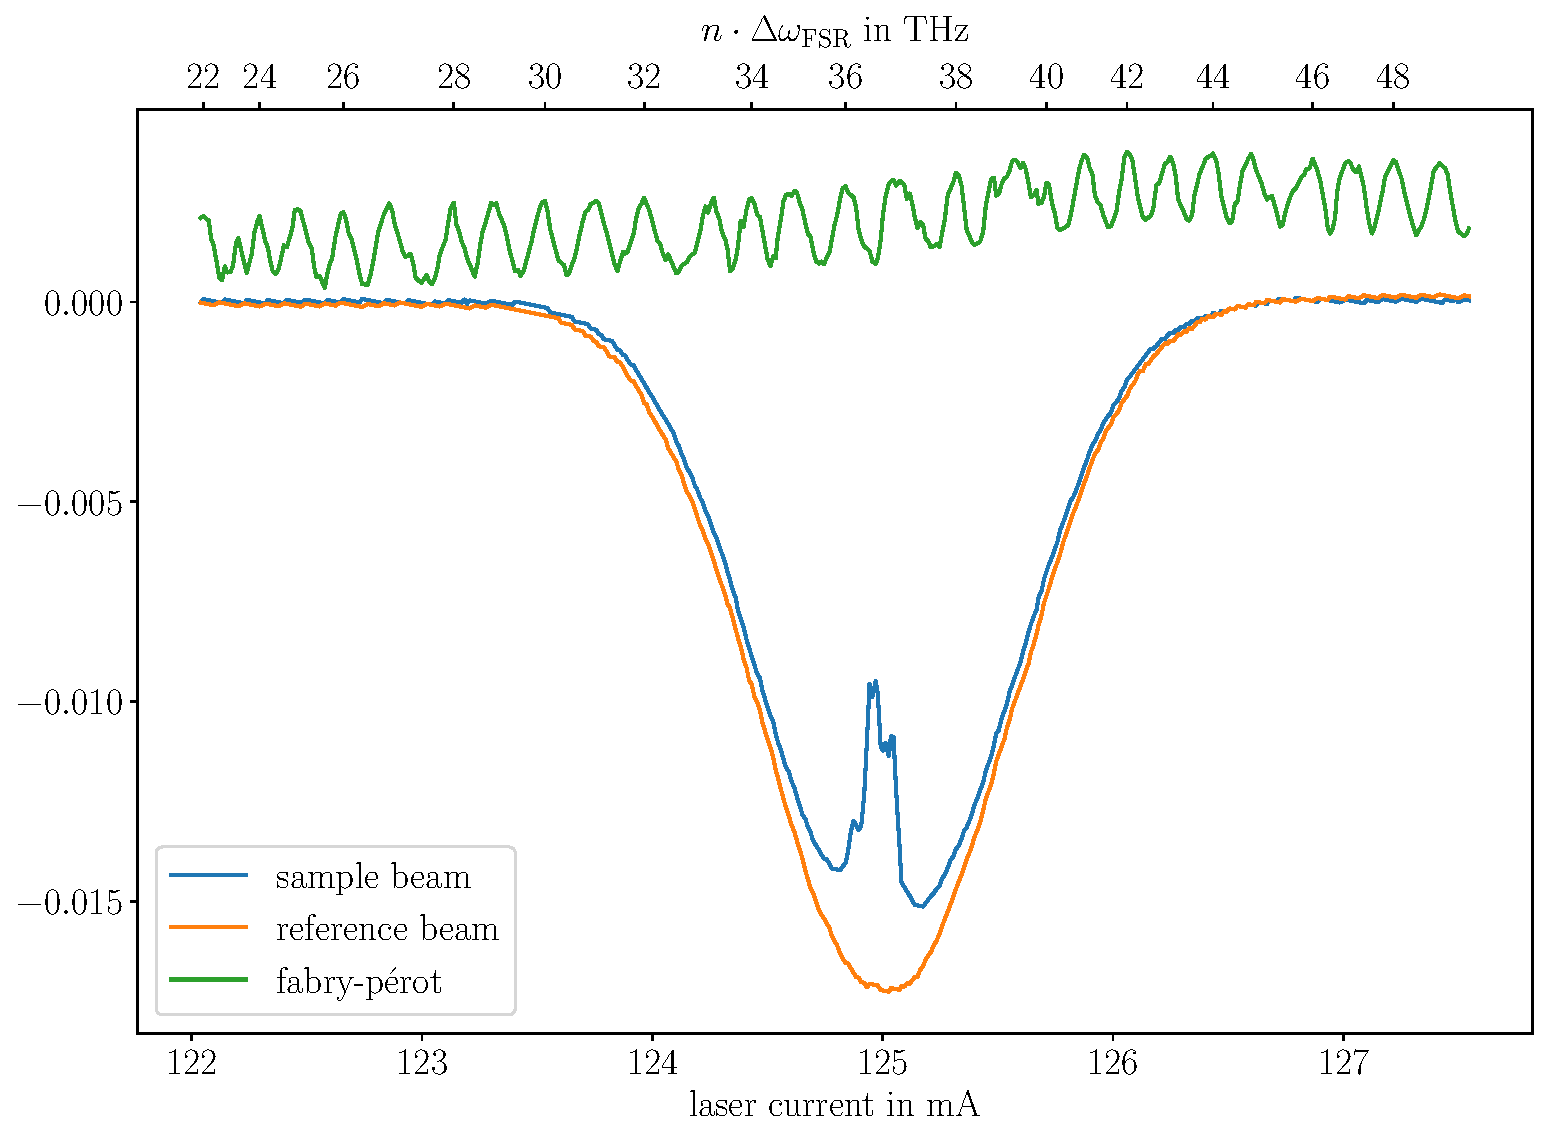
\includegraphics[scale=0.45]{Aufg-4/hyperfine2.pdf}
    \captionof{figure}{absorption spectrum of peak number 2}
    \label{image:peak2}
\end{center}
\begin{center}
    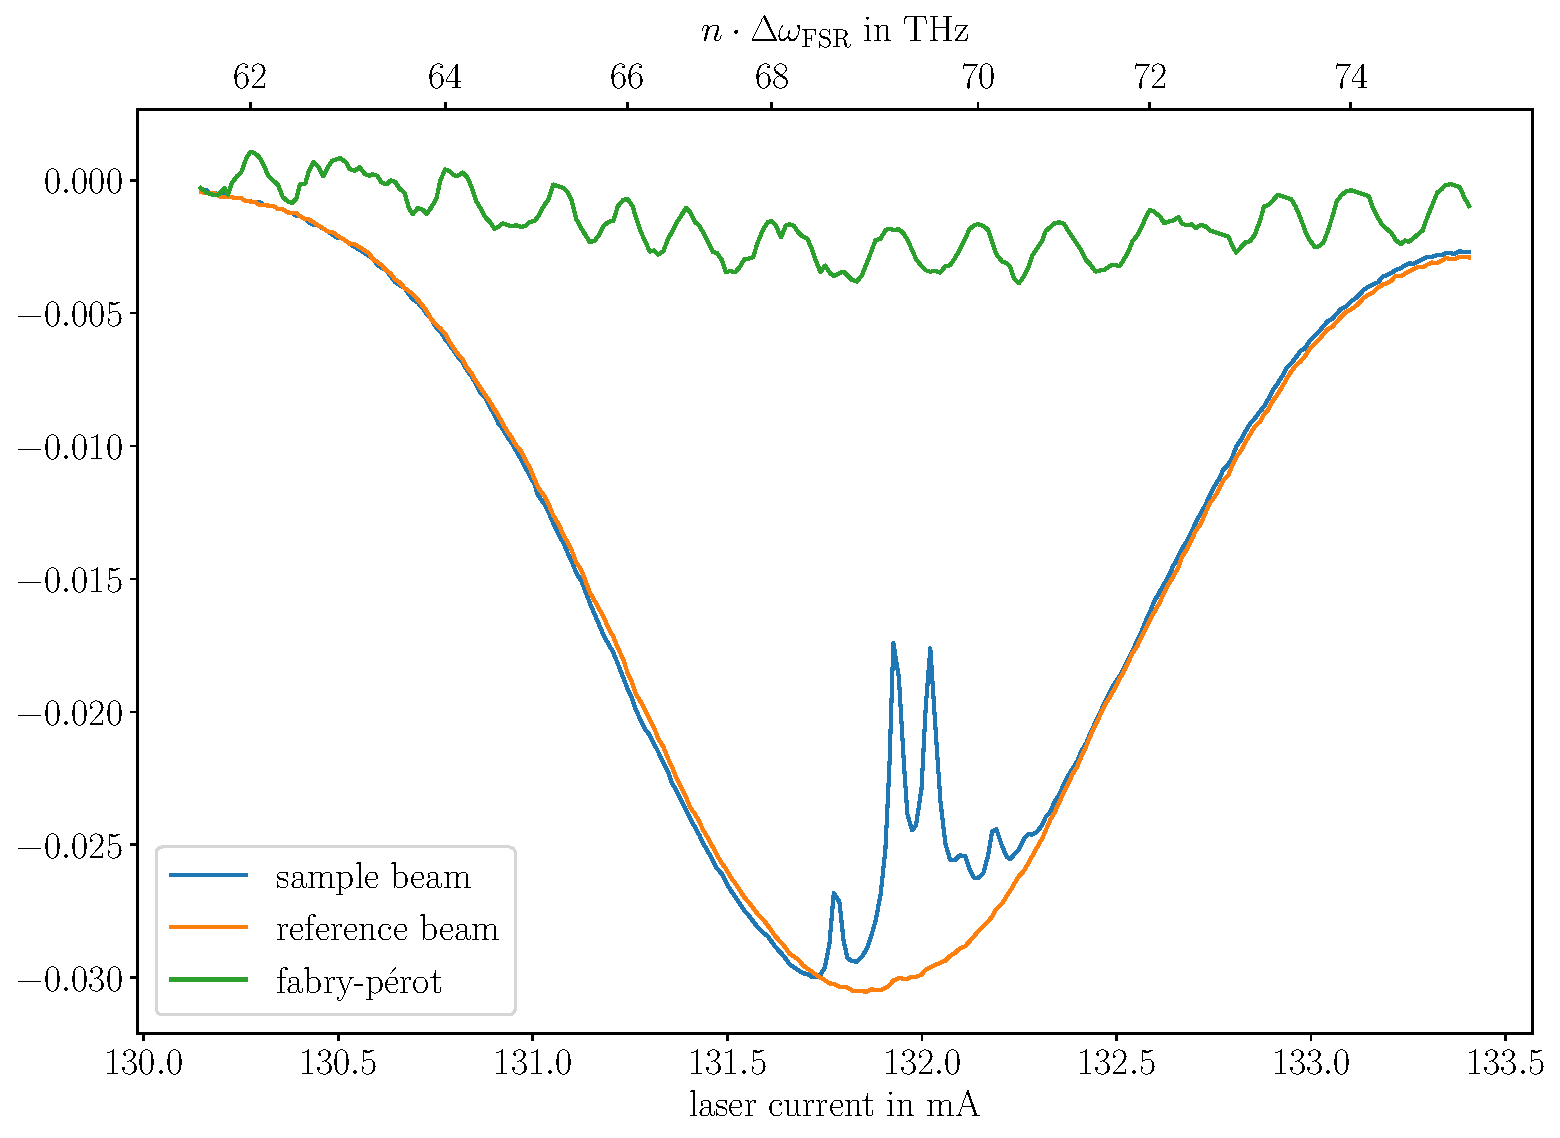
\includegraphics[scale=0.45]{Aufg-4/hyperfine3.pdf}
    \captionof{figure}{absorption spectrum of peak number 3}
    \label{image:peak3}
\end{center}
\begin{center}
    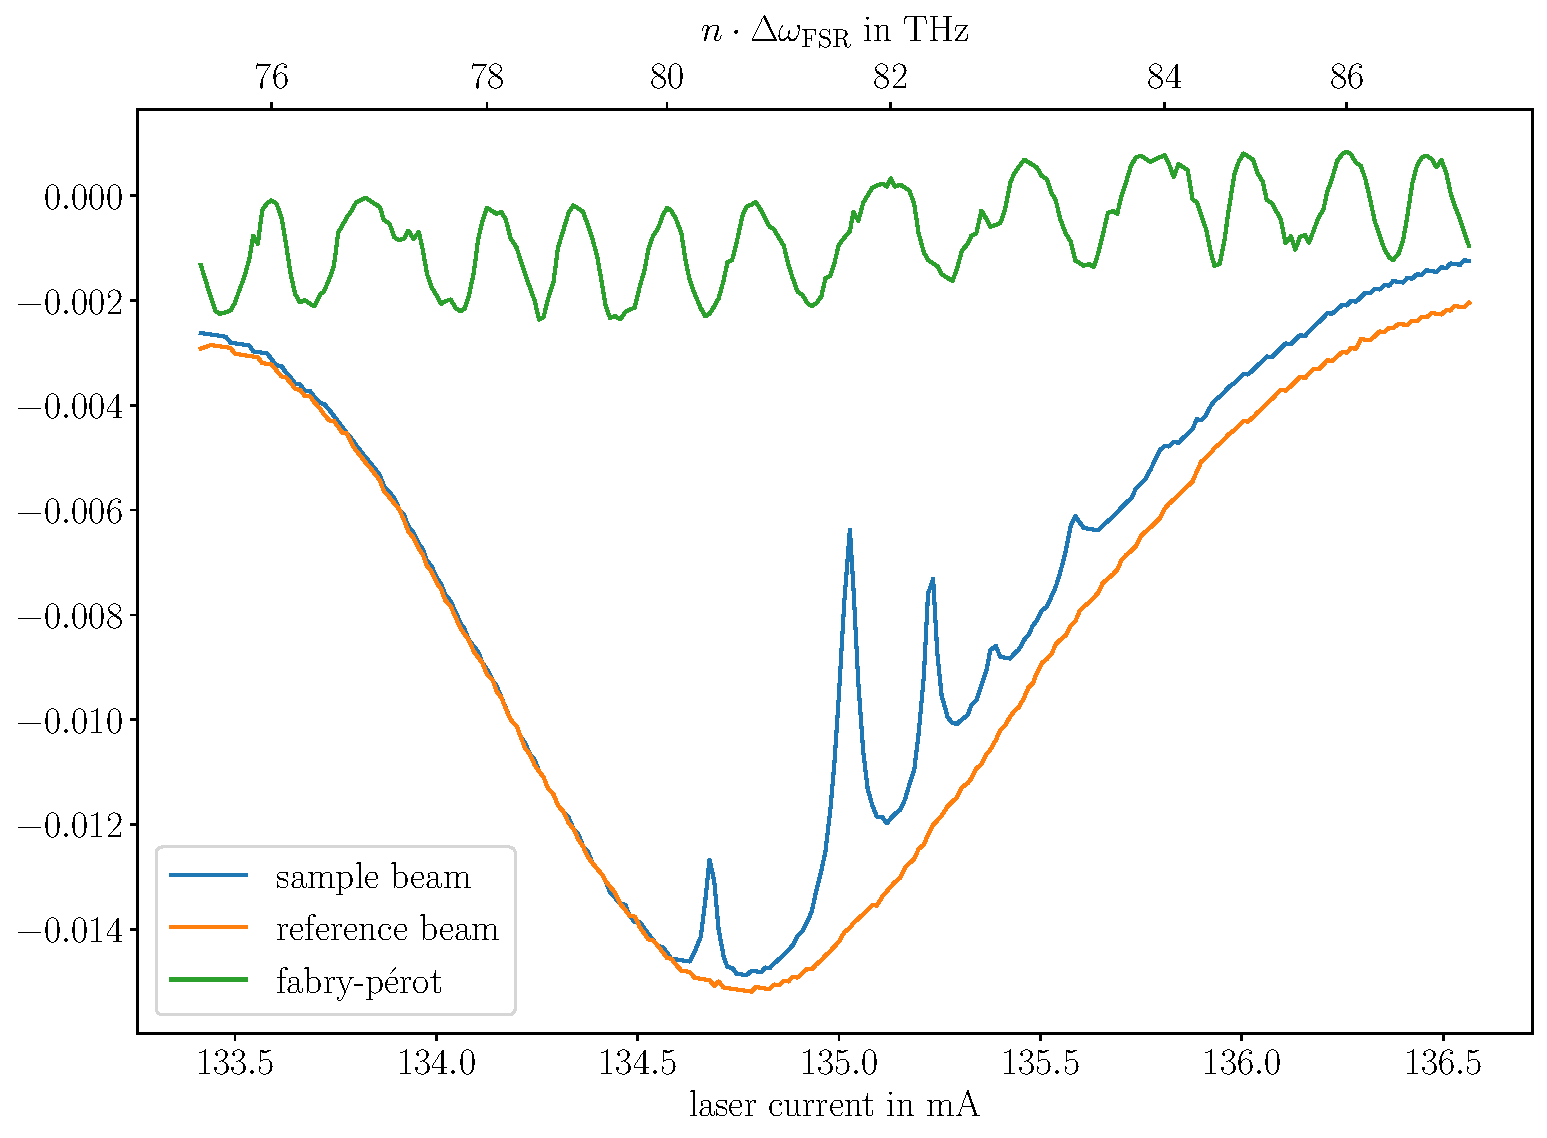
\includegraphics[scale=0.45]{Aufg-4/hyperfine4.pdf}
    \captionof{figure}{absorption spectrum of peak number 4}
    \label{image:peak4}
\end{center}
\newpage
It was chosen to use the peak number 3 because there are the hyperfine dips clearly visible. Its the isotope $^{85}Rb$. For the upcuming calculation we will use the measured data of peak 3 only because of that we have had an offset in our data from $z_{off}=\SI{0.072}{\volt}$ and have to transform the laser current again like in chapter \ref{sec:freeing} into wavelength and frequency.
The fit of the Lorentz curve (lorentzian) was achieved with the function:
\begin{gather}
    y = \frac{a c^2}{(x-b)^2+c^2} - d
\end{gather}
By observing the formula of the fit it gets clear that $a$ is nothing else as the laser current value and $b$ the amplitude of each hyperfine dip peak. From that conclusion we get for the hyperfine peaks numbered from left to right:
\begin{center}
    \begin{tabular}{c | c c c c c c}
        \makecell{hyperfine\\peak} &\makecell{$a$/mA} & $a$/nm &  $a$/THz &  $b$/V & $c$/mA & $d$/V \\
        \hline
        1   &   131.8489  &  780.236290  &  384.232907   &  -0.0269 & -0.0266 & -0.032\\
        2   &   132.0006  &  780.236438  &  384.232834   &  -0.0169 & -0.0285 & -0.032\\
        3   &   132.0778  &  780.236513  &  384.232797   &  -0.0177 & -0.0325 & -0.032\\
        4   &   132.1607  &  780.236594  &  384.232757   &  -0.0254 & -0.0680 & -0.032\\
        5   &   132.2349  &  780.236667  &  384.232722   &  -0.0243 & -0.0613 & -0.032\\
        \end{tabular}
        \captionof{table}{fitting data for each hyperfine dip}
        \label{tab:lorFit}
\end{center}
Furthermore the lorentzian fit for each dip can be seen in fig. \ref{image:lorFit}.\\
It is clear that there are more dips than possible hyperfine transition. In case of $^{85}Rb$ each dip represents a transition from energy levels $F=3$ of the state $5^2S_{1/2}$ to a different energy level of the $5^2P_{3/2}$ state with quantum number $F'$, in short: $F=3\rightarrow F'$. With the selection rule of the hyperfine transition ($\Delta F = 0,\pm1$) we obtain that there should be only three dips visible ($F'=2,3,4$) the remaining dips come from cross over resonances.
For Comparison with the literature \citep{RDL85} we calculate the distance between the dips using table \ref{tab:lorFit} and obtain:
\begin{center}
    \begin{tabular}{c | c c | c c}
        \makecell{dip area} & \makecell{distance\\measured/MHz} & \makecell{distance\\literature/MHz} & \makecell{transition\\ $F'_1\leftrightarrow F'_2$} \\
        \hline
        $1\rightarrow 2$ & 73.00 & 63.38 & $2\leftrightarrow 3$ \\
        $2\rightarrow 5$ & 114.00 & 120.99 & $3\leftrightarrow 4$\\
    \end{tabular}
    \captionof{table}{distance between the selected dips}
    \label{tab:disDip}
\end{center}
The Comparison with the literature shows us that indeed the peek 3 should be $^{85}Rb$ as we assumed in chapter \ref{sec:freeing} and \ref{sec:ratio}. The difference between literature and measurement could have the same cause as the difference in chapter \ref{sec:freeing}.
\newpage
\begin{center}
    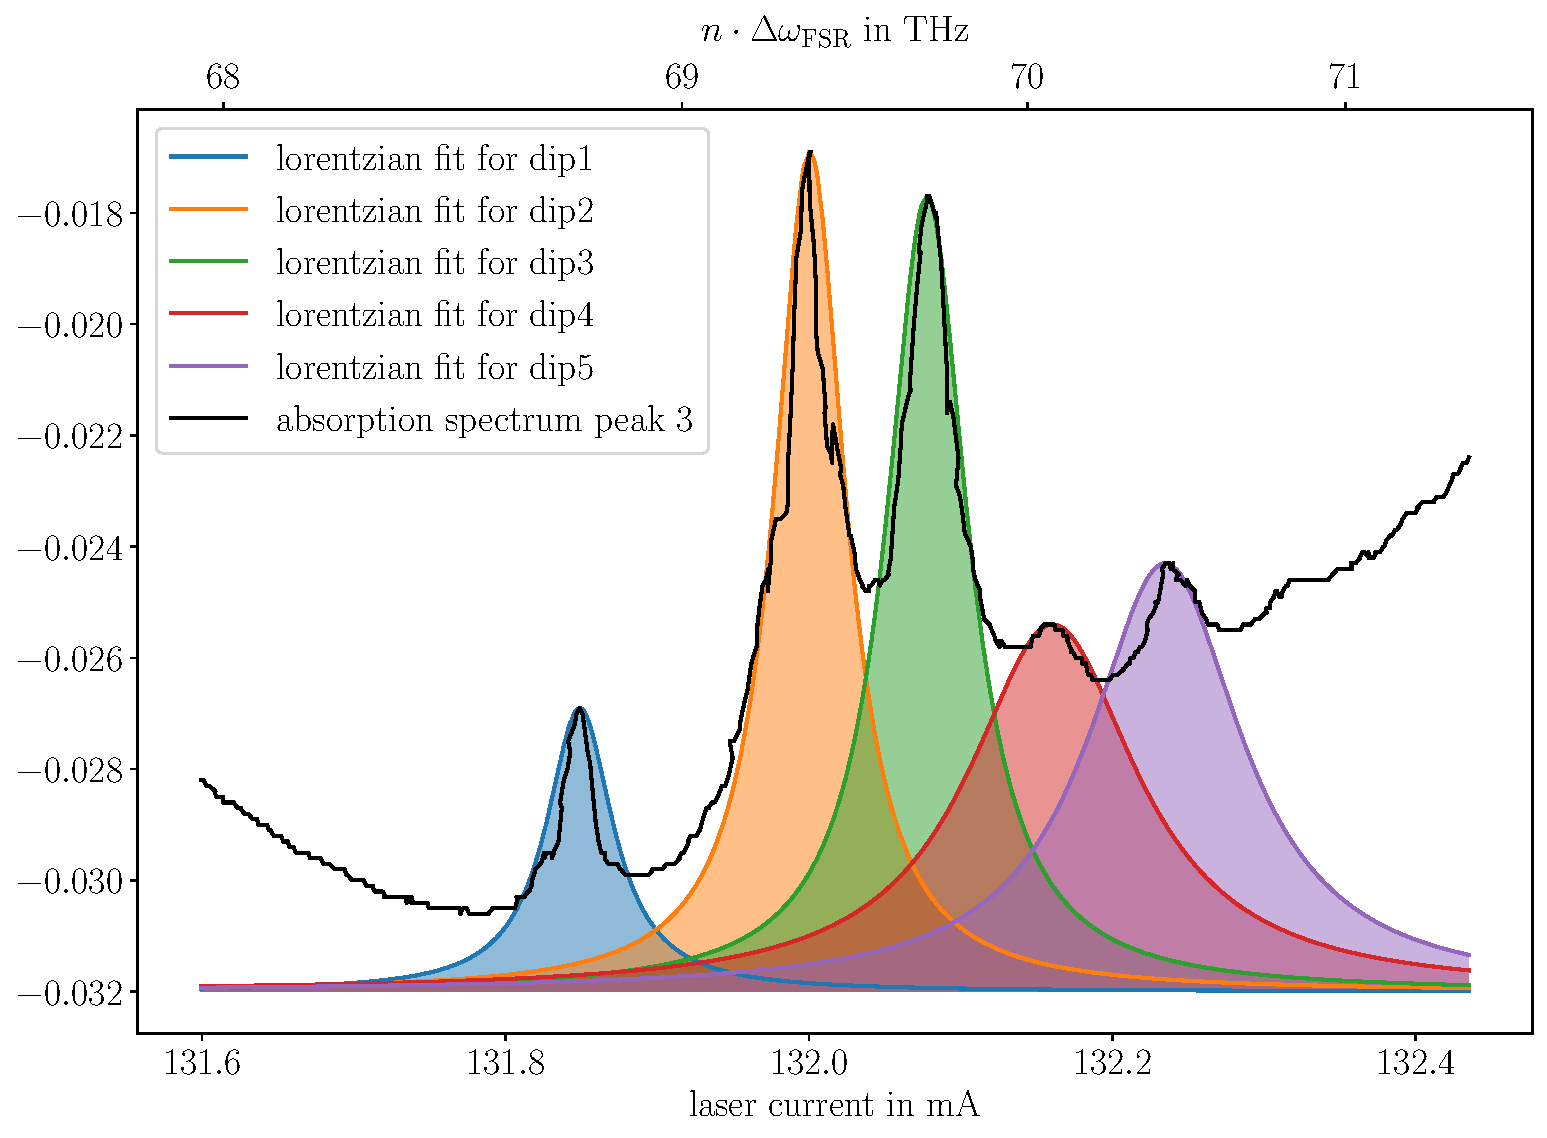
\includegraphics[scale=0.72, angle = 90]{Aufg-4/hyperfinePeak3.pdf}
    \captionof{figure}{lorentzian fit for each dip of peak 3}
    \label{image:lorFit}
\end{center}

%$1\rightarrow 2$ & 73.0 & & \\
%        $2\rightarrow 3$ & 37.0 & & \\
%        $3\rightarrow 4$ & 40.0 & & \\
%        $4\rightarrow 5$ & 37.0 & & \\
\section{Hyperfine constant}
In the following we use the equation \ref{eq:HFS} to calculate the hyperfine constants.
\begin{align}
    \label{eq:HFS}
    \Delta E_{HFS} = \frac{a}{2} [F(F+1) - J(J+1) - I(I+1)]
\end{align}
We know the Energy difference and the Quantum numbers of the transitions from table \ref{tab:disDip}. So we can rewrite the equation: 
\begin{align}
    a = \frac{2(\Delta E)}{F_2(F_2+1)-F_1(F_1+1)} \qquad \text{mit} \quad \Delta E = h \cdot \Delta \nu
\end{align}
After we put in the values we get the following results: 
\begin{table}[h]
    \centering
\begin{tabular}{c|c|c}
    transition & a in $10^{-26}$ J & literature: a in $10^{-26}$ J \\
    \hline
    $2\leftrightarrow 3$ & 1.612 & 1.400\\
    $3\leftrightarrow 4$ & 1.888 & 1.840
\end{tabular}
\caption{hyperfine constants}
\end{table} \\
The literature value of $a$ is computed by the literature value of $\Delta \nu$ from table \ref{tab:disDip}. The difference of one value cloud have the same problem as mentioned in chapter \ref{sec:hyperfine}. 
\newpage
\section{Gas Temperatures}
\label{sec:temp}
To calculate the gas temperature we can use the formula
\begin{gather}
    \Delta \nu_D = \frac{2\nu_0}{c}\sqrt{\ln(2)\frac{2k_BT}{m}} = \frac{2\nu_0\hat{v}}{c}\sqrt{\ln(2)}~\text{with}~\hat{v}= \sqrt{\frac{2k_BT}{m}},
\end{gather}
where $\Delta\nu_D$ is the doppler width, $\nu_0$ the frequency of the peak, $\hat{v}$ the most probable velocity, $k_B$ the Boltzmann constant, $T$ the temperature and $c$ the speed of light in vacuum.
First we have to calculate the doppler width or most probable velocity. For that we are fitting a gaussian on the spectrum of the reference beam as in chapter \ref{image:gaussFit} with the form:
\begin{gather}
    y = y(\nu_0) \exp(-\left(\frac{\nu-\nu_0}{\sigma}\right)^2)
\end{gather}
With the value of $\sigma$ one can calculate $\Delta\nu_D$ or $\hat{v}$ as following:
\begin{gather}
    \Delta\nu_D = 2\sqrt{\ln(2)}\sigma \Rightarrow \sigma = \frac{\nu_0\hat{v}}{c} \Leftrightarrow \hat{v} = \frac{\sigma c}{\nu_0}
\end{gather}
After that one can obtain $T$ and the mean velocity $\overline{v}$:
\begin{gather}
    \hat{v} =  \sqrt{\frac{2k_BT}{m}} \Leftrightarrow T = \frac{m}{2 k_B} \hat{v}^2~\text{and}~\overline{v} = \sqrt{\frac{8k_BT}{\pi m}} = \sqrt{\frac{4}{\pi}}\cdot\hat{v}
\end{gather} 
We selected peak 2 for the upcoming calculation for each temperature. Because of the previous chapters \ref{sec:freeing} and \ref{sec:ratio} we know that peak 2 have to be $^{87}Rb$ and so the mass is $m\approx1.44322\cdot 10^{-25}$kg. We have transformed the laser current into frequency as in chapter \ref{sec:freeing} and with the knowledge of $\sigma$ we get following table:
\begin{center}
    \begin{tabular}{r | c c c| c c | c c}
        Temp & $\nu_0$/THz & $y(\nu_0)$/V & $\sigma$/MHz & $\hat{v}$/$\frac{m}{s}$ & $\overline{v}$/$\frac{m}{s}$& $T$/K & $T_{act}$/K\\
        \hline 
        \SI{24}{\celsius}   &384.22713 & -0.0173 & 345.26881 & 269.40 & 303.98 & 379.31 & 297,15\\ 
        \SI{38}{\celsius}   &384.22737 & -0.0313 & 361.10835 & 281.75 & 317.93 & 414.91 & 313,15\\ 
        \SI{56.2}{\celsius} &384.22724 & -0.0482 & 398.62826 & 311.03 & 350.96 & 505.62 & 329,35\\ 
    \end{tabular}
    \captionof{table}{fit parameter, velocities and temperature of the gas for each acted temperature}
\end{center}
It appears that the calculated temperatures for the gas differs from the acting temperature. But it is worth noticing that the value for $\sigma$ and so also the doppler width $\Delta\nu_D$ increases with higher temperature. In conclusion to that it gets clear that the scale of the measured values is right and that the transformation from current to frequency once again has cause problems in determine the gas temperature accurately.\\

Lastly we show in fig. \ref{image:gaussFit24}, \ref{image:gaussFit38} and \ref{image:gaussFit56} gaussian fit for each temperature.
\begin{center}
    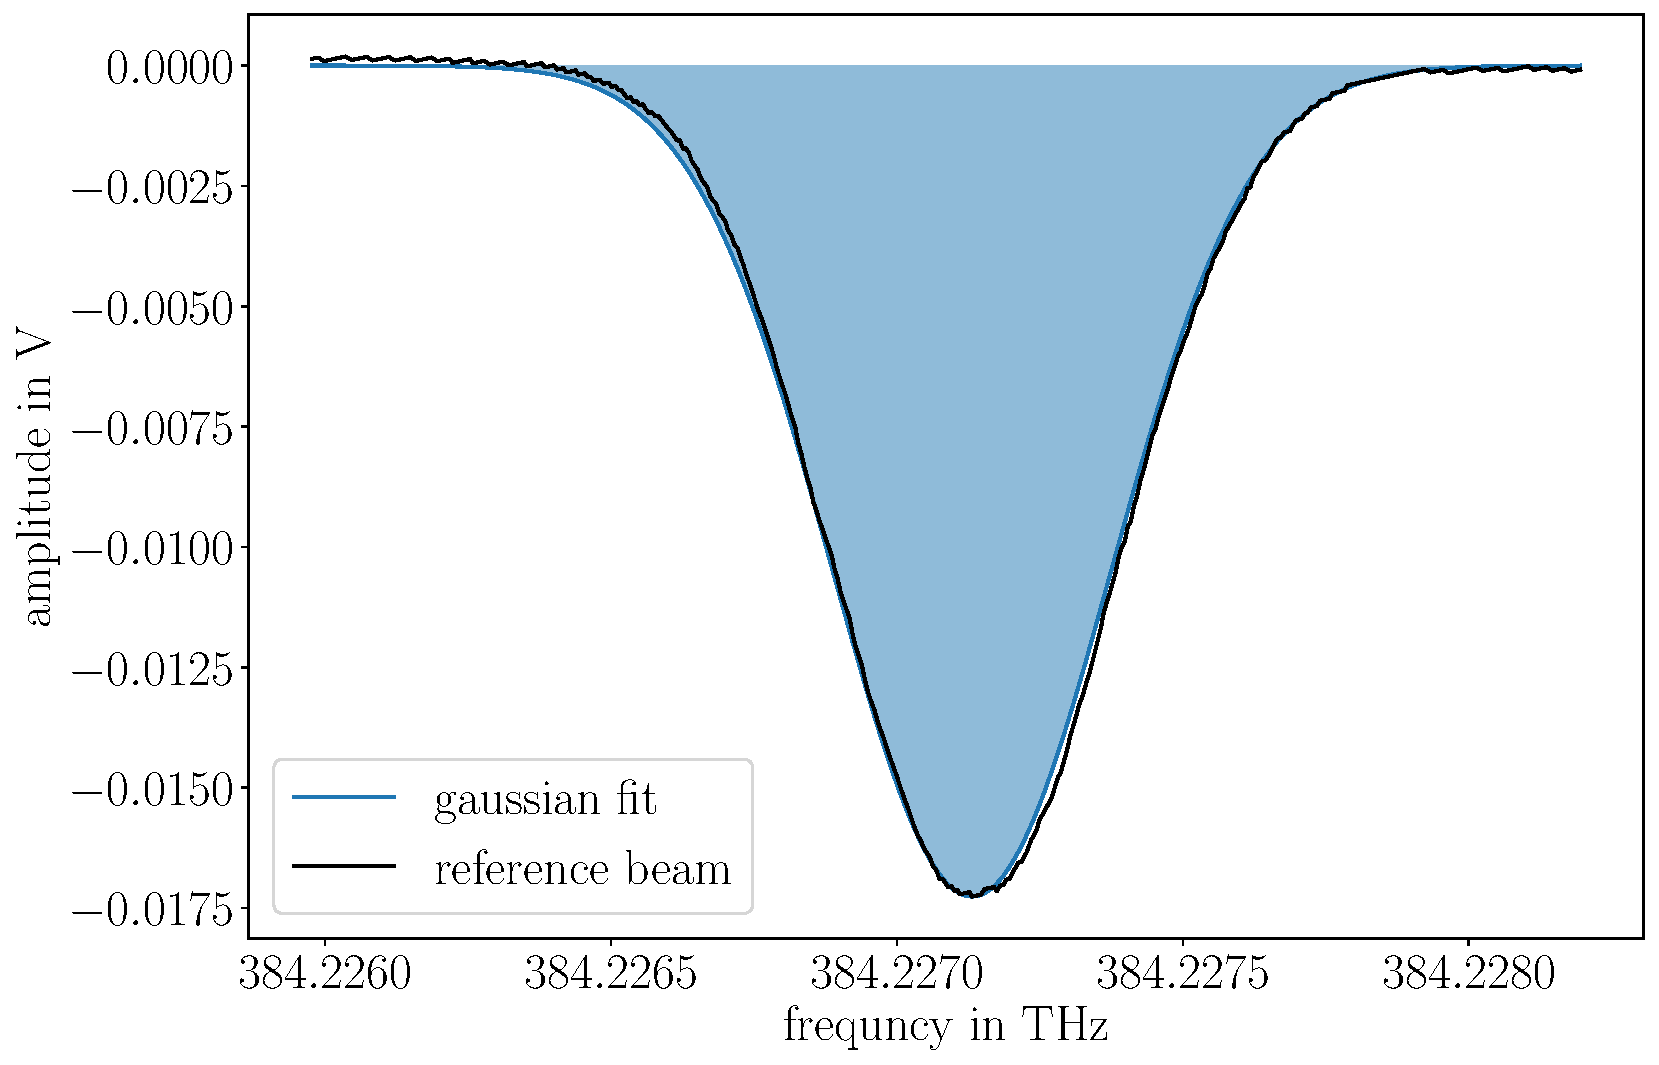
\includegraphics[scale = 0.3]{Aufg-5/gaussFitTemp24.pdf}
    \captionof{figure}{gaussian fit for temperature \SI{24}{\celsius}}
    \label{image:gaussFit24}
\end{center}
\begin{center}
    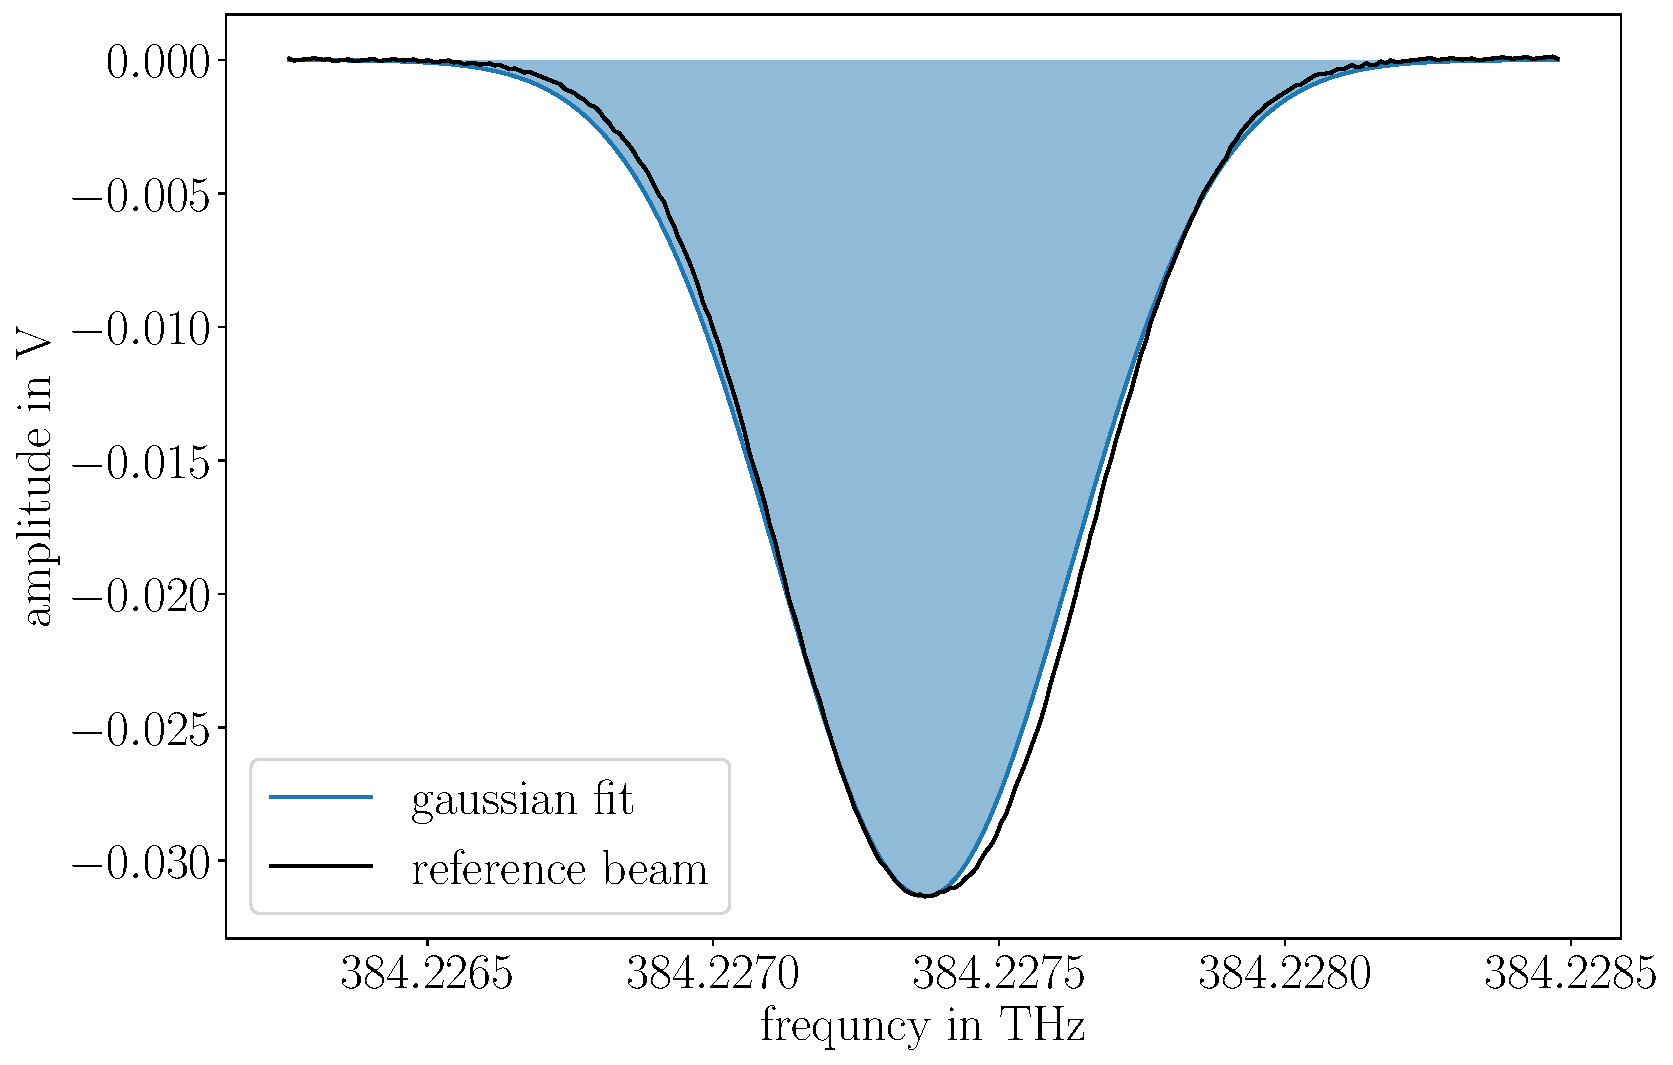
\includegraphics[scale = 0.3]{Aufg-5/gaussFitTemp38.pdf}
    \captionof{figure}{gaussian fit for temperature \SI{38}{\celsius}}
    \label{image:gaussFit38}
\end{center}
\begin{center}
    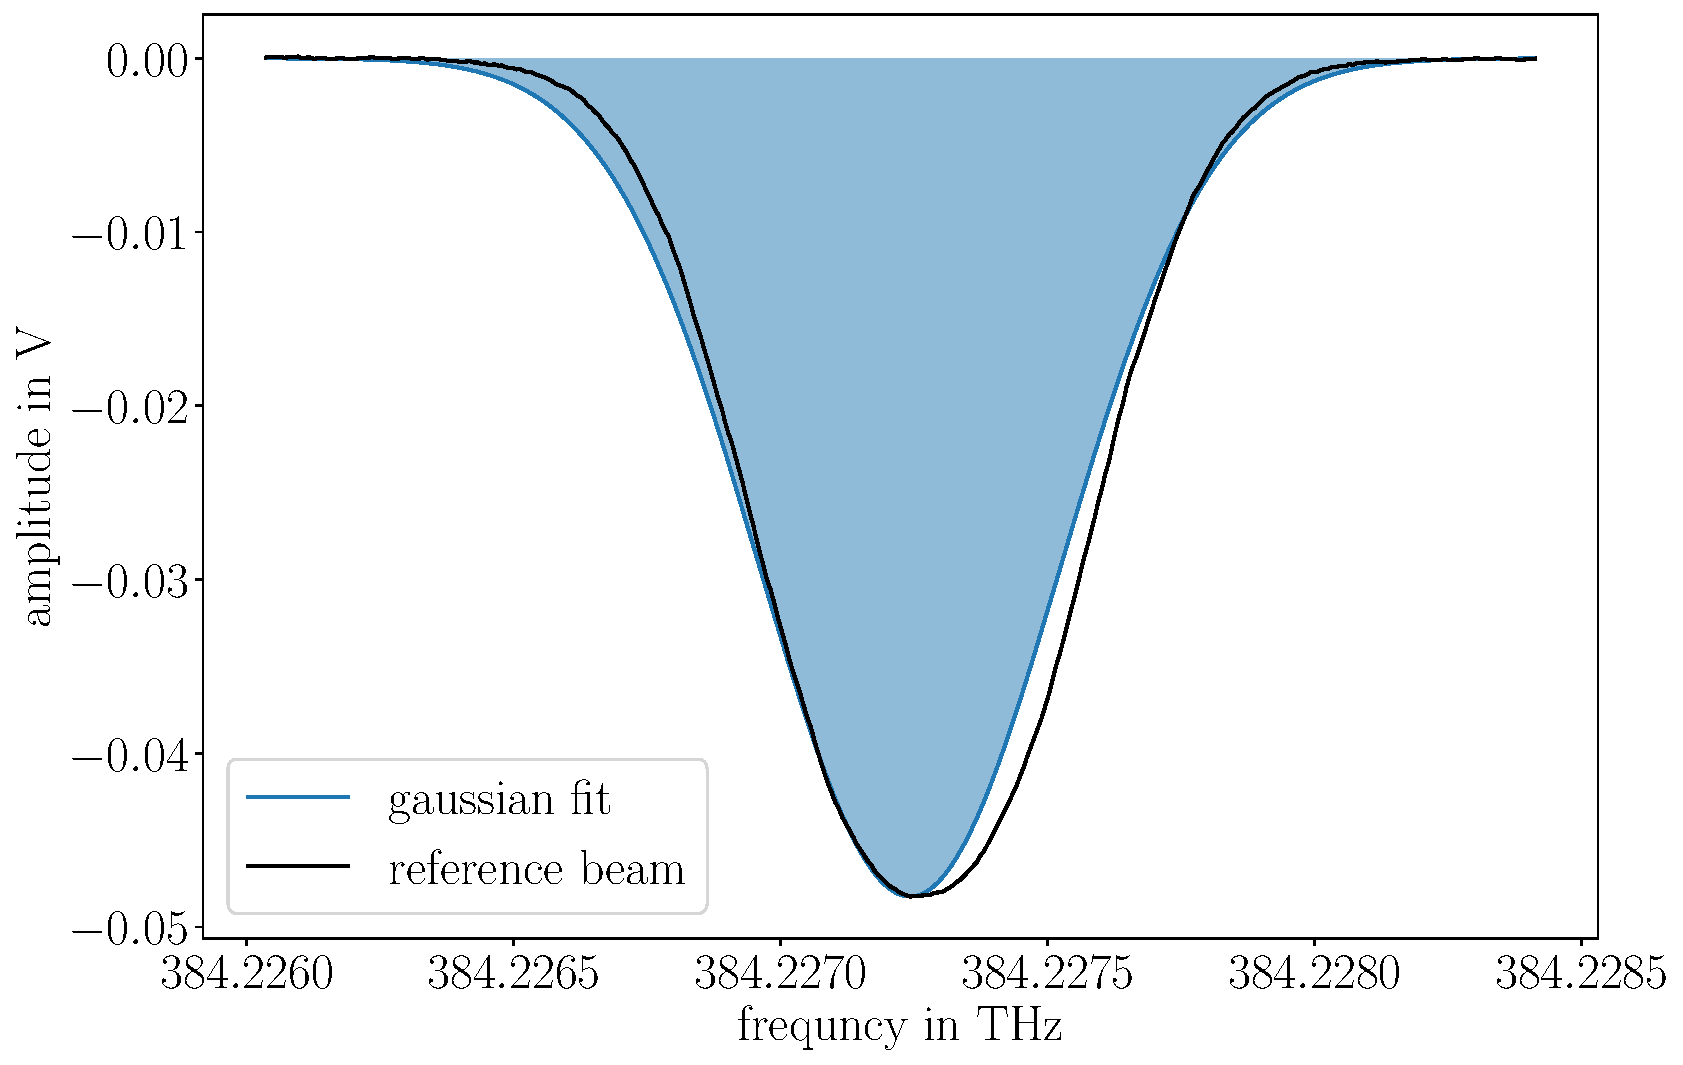
\includegraphics[scale = 0.3]{Aufg-5/gaussFitTemp56.pdf}
    \captionof{figure}{gaussian fit for temperature \SI{56.2}{\celsius}}
    \label{image:gaussFit56}
\end{center}

% etc.

    % 5.Chapter Closure
    % 5. Closure

\chapter{Closure}
\label{chap:close}

In the experiment and the following evaluation of the measured data it becomes clear that the measurement have to be very precisely to detect the small transitions for the hyperfine structure. In the evaluation itself we learned how to fit functions on our measured data, and we get a good overview in the handling of precise measured data.\\
Overall this experiment gave us a good insight into the topic of saturation spectroscopy and it was a pleasure to see how theory becomes reality.

    % Appendix
    %% Appendix

\appendix

% Text

% Charlotte Geiger - Manuel Lippert - Leonard Schatt
% Physikalisches Praktikum

% Anhang A

\chapter{Berechnungen Fourier-Reihenkoeffizient und Effektivspannung}
\label{app:Berechnung}

\section*{Sinusschwingung}
Effektivspannung:
\begin{gather}
    U_{eff} = \sqrt{\frac{1}{T}\int^T_0 U_0^2 \sin^2\left(\frac{2\pi}{T}\right) dt} = \sqrt{\frac{U_0^2}{T} \left[\frac{t}{2} - \frac{T\sin(\frac{4\pi}{T}t)}{8\pi}\bigg \vert^T_0 \right]} = \sqrt{\frac{U_0^2}{T}\frac{T}{2}} = \frac{U_0}{\sqrt{2}}
\end{gather}

\section*{Rechteckschwingung}
$b_k$ der Fourier-Reihe:
\begin{gather}
    \begin{aligned}
        b_k &= \frac{2}{T} \int^{T}_{0} f(t)\sin(k \frac{2\pi}{T} t)dt\\
            &= \frac{2}{T} \left[ \int^{\frac{T}{2}}_{0} U_0\sin(k \frac{2\pi}{T} t)dt - \int^{T}_{\frac{T}{2}} U_0\sin(k \frac{2\pi}{T} t)dt\right]\\
            &= \frac{2}{T}\frac{U_0T}{k2\pi} \left[-\cos(k \frac{2\pi}{T} t) \bigg \vert^{\frac{T}{2}}_{0} + \cos(k \frac{2\pi}{T} t) \bigg \vert^{T}_{\frac{T}{2}} \right]\\
            &= \frac{U_0}{k\pi} \left[-\cos(k\pi)+1 + 1 - \cos(k\pi)\right]\\
            &= \frac{2U_0}{k\pi}\left[1-\cos(k\pi)\right]
    \end{aligned}\\[0,5cm]
    \Rightarrow b_k =
    \begin{cases}
        0, & k~\text{gerade}\\
        \frac{4U_0}{\pi}\frac{1}{k}, & k~\text{ungerade}\\
    \end{cases}
\end{gather}

Effektivspannung:
\begin{gather}
    U_{eff} = \sqrt{\frac{1}{T}\left[\int^{\frac{T}{2}}_0 U_0^2dt + \int^T_{\frac{T}{2}} U_0^2 dt\right]} = \sqrt{\frac{U_0^2}{T}\left[\frac{T}{2}+T-\frac{T}{2}\right]} = U_0
\end{gather}

\section*{Dreiecksschwingung}
$b_k$ der Fourier-Reihe:
\begin{gather}
    \begin{aligned}
        b_k &= \frac{2}{T} \int^{\frac{3T}{4}}_{-\frac{T}{4}} f(t)\sin(k \frac{2\pi}{T} t)dt\\
            &= \frac{2}{T} \left[\int^{\frac{T}{4}}_{-\frac{T}{4}} at\sin(k \frac{2\pi}{T} t)dt+ \int^{\frac{3T}{4}}_{\frac{T}{4}} a\left(\frac{T}{2}-t\right)\sin(k \frac{2\pi}{T} t)dt\right]\\
            &= \frac{2a}{T} \left[\int^{\frac{T}{4}}_{-\frac{T}{4}} t\sin(k \frac{2\pi}{T} t)dt - \int^{\frac{3T}{4}}_{\frac{T}{4}}t\sin(k \frac{2\pi}{T} t)dt\right] + \int^{\frac{3T}{4}}_{\frac{T}{4}}a\sin(k \frac{2\pi}{T} t)dt\\
            &= (\text{I}) + (\text{II})\\[0,5cm]
        (\text{I}) &= \frac{2a}{T} \left[\int^{\frac{T}{4}}_{-\frac{T}{4}} t\sin(k \frac{2\pi}{T} t)
            dt - \int^{\frac{3T}{4}}_{\frac{T}{4}}t\sin(k \frac{2\pi}{T} t)dt\right] \Rightarrow~\text{Partielle Integration}\\
            &= \frac{2a}{T}\frac{T}{k2\pi} \left[-t\cos(k \frac{2\pi}{T} t) \bigg \vert^{\frac{T}{4}}_{-\frac{T}{4}} + t\cos(k \frac{2\pi}{T} t) \bigg \vert^{\frac{3T}{4}}_{\frac{T}{4}}\right]\\
            &\tab+\frac{2a}{T}\frac{T}{k2\pi}\left[\int^{\frac{T}{4}}_{-\frac{T}{4}} \cos(k \frac{2\pi}{T} t)dt - \int^{\frac{3T}{4}}_{\frac{T}{4}} \cos(k \frac{2\pi}{T} t)dt\right]\\
            &= \frac{2a}{T}\frac{T}{k2\pi} \left[-\frac{T}{4}\cos(k \frac{\pi}{2}) -\frac{T}{4}\cos(- k \frac{\pi}{2}) + \frac{3T}{4} \cos(k \frac{3\pi}{2}) - \frac{T}{4} \cos(k \frac{\pi}{2}) \right]\\
            &\tab+\frac{2a}{T}\frac{T}{k2\pi}\left[\int^{\frac{T}{4}}_{-\frac{T}{4}} \cos(k \frac{2\pi}{T} t)dt - \int^{\frac{3T}{4}}_{\frac{T}{4}} \cos(k \frac{2\pi}{T} t)dt\right]\\
            &= \frac{2a}{T}\frac{T}{k2\pi}\left[\int^{\frac{T}{4}}_{-\frac{T}{4}} \cos(k \frac{2\pi}{T} t)dt - \int^{\frac{3T}{4}}_{\frac{T}{4}} \cos(k \frac{2\pi}{T} t)dt\right]\\
            &= \frac{2a}{T}\left(\frac{T}{k2\pi}\right)^2 \left[\sin(k \frac{2\pi}{T} t) \bigg \vert^{\frac{T}{4}}_{-\frac{T}{4}} - \sin(k \frac{2\pi}{T} t) \bigg \vert^{\frac{3T}{4}}_{\frac{T}{2}}\right]\\
            &= \frac{2a}{T}\left(\frac{T}{k2\pi}\right)^2 \left[\sin(k\frac{\pi}{2}) - \sin(-k\frac{\pi}{2}) - \sin(k\frac{3\pi}{2}) + \sin(k\frac{\pi}{2})\right]\\[0,5cm]
        (\text{II}) &= \int^{\frac{3T}{4}}_{\frac{T}{4}}a\sin(k \frac{2\pi}{T} t)dt = \frac{aT}{2\pi} \left[\cos(k\frac{2\pi}{T}t)\bigg \vert^{\frac{3T}{4}}_{\frac{T}{4}}\right]\\
                    &= \frac{aT}{2\pi} \left[\cos(k\frac{3\pi}{2}) - \cos(k\frac{\pi}{2})\right] = 0
    \end{aligned}\\[0,5cm]
    \Rightarrow b_k =
    \begin{cases}
        0, & k~\text{gerade}\\
        \frac{8aT}{4\pi^2}\frac{(-1)^{k-1}}{k^2} = \frac{8U_0}{\pi^2}\frac{(-1)^{k-1}}{k^2}, & k~\text{ungerade}\\
    \end{cases}
\end{gather}
Effektivspannung:
\begin{gather}
    \begin{aligned}
        U_{eff} &= \sqrt{\frac{1}{T}\left[\int^{\frac{T}{4}}_{-\frac{T}{4}} (at)^2dt + \int^{\frac{3T}{4}}_{\frac{T}{4}} \left(a\left(\frac{T}{2}-t\right)\right)^2 dt\right]}\\
                &= \sqrt{\frac{a^2}{T}\left[\int^{\frac{T}{4}}_{-\frac{T}{4}} t^2dt + \int^{\frac{3T}{4}}_{\frac{T}{4}} \left(\frac{T}{2}-t\right)^2 dt\right]}
                = \sqrt{\frac{a^2}{3T}\left[t^3 \bigg \vert^{\frac{T}{4}}_{-\frac{T}{4}} - \left(\frac{T}{2}-t\right)^3 \bigg \vert^{\frac{3T}{4}}_{\frac{T}{4}}\right]}\\
                &= \sqrt{\frac{a^2}{3T}\left[\left(\frac{T}{4}\right)^3 + \left(\frac{T}{4}\right)^3 - \left(\frac{T}{2}- \frac{3T}{4} \right)^3 +  \left(\frac{T}{2}- \frac{T}{4} \right)^3\right]}\\
                &= \sqrt{\frac{a^2}{3T}\left(\frac{T^3}{16}\right)} = \sqrt{\frac{1}{3}\left(\frac{aT}{4}\right)^2} = \sqrt{\frac{U_0^2}{3}} = \frac{U_0}{\sqrt{3}}
     \end{aligned}
\end{gather}


    % Literatur
    \bibliographystyle{Auswertung.bst}
    \bibliography{Auswertung.bib}
    
\end{document}